\documentclass[twoside]{book}

% Packages required by doxygen
\usepackage{calc}
\usepackage{doxygen}
\usepackage{graphicx}
\usepackage[utf8]{inputenc}
\usepackage{makeidx}
\usepackage{multicol}
\usepackage{multirow}
\usepackage{textcomp}
\usepackage[table]{xcolor}

% Font selection
\usepackage[T1]{fontenc}
\usepackage{mathptmx}
\usepackage[scaled=.90]{helvet}
\usepackage{courier}
\usepackage{amssymb}
\usepackage{sectsty}
\renewcommand{\familydefault}{\sfdefault}
\allsectionsfont{%
  \fontseries{bc}\selectfont%
  \color{darkgray}%
}
\renewcommand{\DoxyLabelFont}{%
  \fontseries{bc}\selectfont%
  \color{darkgray}%
}

% Page & text layout
\usepackage{geometry}
\geometry{%
  a4paper,%
  top=2.5cm,%
  bottom=2.5cm,%
  left=2.5cm,%
  right=2.5cm%
}
\tolerance=750
\hfuzz=15pt
\hbadness=750
\setlength{\emergencystretch}{15pt}
\setlength{\parindent}{0cm}
\setlength{\parskip}{0.2cm}
\makeatletter
\renewcommand{\paragraph}{%
  \@startsection{paragraph}{4}{0ex}{-1.0ex}{1.0ex}{%
    \normalfont\normalsize\bfseries\SS@parafont%
  }%
}
\renewcommand{\subparagraph}{%
  \@startsection{subparagraph}{5}{0ex}{-1.0ex}{1.0ex}{%
    \normalfont\normalsize\bfseries\SS@subparafont%
  }%
}
\makeatother

% Headers & footers
\usepackage{fancyhdr}
\pagestyle{fancyplain}
\fancyhead[LE]{\fancyplain{}{\bfseries\thepage}}
\fancyhead[CE]{\fancyplain{}{}}
\fancyhead[RE]{\fancyplain{}{\bfseries\leftmark}}
\fancyhead[LO]{\fancyplain{}{\bfseries\rightmark}}
\fancyhead[CO]{\fancyplain{}{}}
\fancyhead[RO]{\fancyplain{}{\bfseries\thepage}}
\fancyfoot[LE]{\fancyplain{}{}}
\fancyfoot[CE]{\fancyplain{}{}}
\fancyfoot[RE]{\fancyplain{}{\bfseries\scriptsize Generated on Thu Apr 24 2014 13:00:40 for SLAM by Doxygen }}
\fancyfoot[LO]{\fancyplain{}{\bfseries\scriptsize Generated on Thu Apr 24 2014 13:00:40 for SLAM by Doxygen }}
\fancyfoot[CO]{\fancyplain{}{}}
\fancyfoot[RO]{\fancyplain{}{}}
\renewcommand{\footrulewidth}{0.4pt}
\renewcommand{\chaptermark}[1]{%
  \markboth{#1}{}%
}
\renewcommand{\sectionmark}[1]{%
  \markright{\thesection\ #1}%
}

% Indices & bibliography
\usepackage{natbib}
\usepackage[titles]{tocloft}
\setcounter{tocdepth}{3}
\setcounter{secnumdepth}{5}
\makeindex

% Custom commands
\newcommand{\clearemptydoublepage}{%
  \newpage{\pagestyle{empty}\cleardoublepage}%
}


%===== C O N T E N T S =====

\begin{document}

% Titlepage & ToC
\pagenumbering{roman}
\begin{titlepage}
\vspace*{7cm}
\begin{center}%
{\Large S\-L\-A\-M }\\
\vspace*{1cm}
{\large Generated by Doxygen 1.8.4}\\
\vspace*{0.5cm}
{\small Thu Apr 24 2014 13:00:40}\\
\end{center}
\end{titlepage}
\clearemptydoublepage
\tableofcontents
\clearemptydoublepage
\pagenumbering{arabic}

%--- Begin generated contents ---
\chapter{Namespace Index}
\section{Packages}
Here are the packages with brief descriptions (if available)\-:\begin{DoxyCompactList}
\item\contentsline{section}{{\bf S\-L\-A\-M} }{\pageref{namespace_s_l_a_m}}{}
\end{DoxyCompactList}

\chapter{Hierarchical Index}
\section{Class Hierarchy}
This inheritance list is sorted roughly, but not completely, alphabetically\-:\begin{DoxyCompactList}
\item Drawing\-Area\begin{DoxyCompactList}
\item \contentsline{section}{S\-L\-A\-M.\-Map\-View}{\pageref{class_s_l_a_m_1_1_map_view}}{}
\end{DoxyCompactList}
\item \contentsline{section}{S\-L\-A\-M.\-Ekf\-Slam}{\pageref{class_s_l_a_m_1_1_ekf_slam}}{}
\item Event\-Args\begin{DoxyCompactList}
\item \contentsline{section}{S\-L\-A\-M.\-Map\-Update\-Event\-Args}{\pageref{class_s_l_a_m_1_1_map_update_event_args}}{}
\item \contentsline{section}{S\-L\-A\-M.\-Robot\-Update\-Event\-Args}{\pageref{class_s_l_a_m_1_1_robot_update_event_args}}{}
\end{DoxyCompactList}
\item \contentsline{section}{S\-L\-A\-M.\-Landmark}{\pageref{class_s_l_a_m_1_1_landmark}}{}
\item \contentsline{section}{S\-L\-A\-M.\-Landmark\-View}{\pageref{class_s_l_a_m_1_1_landmark_view}}{}
\item \contentsline{section}{S\-L\-A\-M.\-Path\-View}{\pageref{class_s_l_a_m_1_1_path_view}}{}
\item \contentsline{section}{S\-L\-A\-M.\-Robot}{\pageref{class_s_l_a_m_1_1_robot}}{}
\item \contentsline{section}{S\-L\-A\-M.\-Robot\-View}{\pageref{class_s_l_a_m_1_1_robot_view}}{}
\item \contentsline{section}{S\-L\-A\-M.\-S\-L\-A\-M}{\pageref{class_s_l_a_m_1_1_s_l_a_m}}{}
\item \contentsline{section}{S\-L\-A\-M.\-Slam\-Map}{\pageref{class_s_l_a_m_1_1_slam_map}}{}
\item Window\begin{DoxyCompactList}
\item \contentsline{section}{S\-L\-A\-M.\-Map\-Window}{\pageref{class_s_l_a_m_1_1_map_window}}{}
\end{DoxyCompactList}
\end{DoxyCompactList}

\chapter{Class Index}
\section{Class List}
Here are the classes, structs, unions and interfaces with brief descriptions\-:\begin{DoxyCompactList}
\item\contentsline{section}{{\bf S\-L\-A\-M.\-Ekf\-Slam} \\*Summary description for Landmarks. }{\pageref{class_s_l_a_m_1_1_ekf_slam}}{}
\item\contentsline{section}{{\bf S\-L\-A\-M.\-Landmark} \\*\doxyref{Landmark}{p.}{class_s_l_a_m_1_1_landmark}. }{\pageref{class_s_l_a_m_1_1_landmark}}{}
\item\contentsline{section}{{\bf S\-L\-A\-M.\-Landmark\-View} \\*\doxyref{Landmark}{p.}{class_s_l_a_m_1_1_landmark} view. }{\pageref{class_s_l_a_m_1_1_landmark_view}}{}
\item\contentsline{section}{{\bf S\-L\-A\-M.\-Map\-Update\-Event\-Args} \\*An event to handle any updates to the map. }{\pageref{class_s_l_a_m_1_1_map_update_event_args}}{}
\item\contentsline{section}{{\bf S\-L\-A\-M.\-Map\-View} \\*Map view. }{\pageref{class_s_l_a_m_1_1_map_view}}{}
\item\contentsline{section}{{\bf S\-L\-A\-M.\-Map\-Window} \\*Map window. }{\pageref{class_s_l_a_m_1_1_map_window}}{}
\item\contentsline{section}{{\bf S\-L\-A\-M.\-Path\-View} \\*Path view. Keeps Track of where the robot has been visually on the map }{\pageref{class_s_l_a_m_1_1_path_view}}{}
\item\contentsline{section}{{\bf S\-L\-A\-M.\-Robot} \\*Contains the exploration robot model as part of the Model-\/\-View-\/\-Controller (M\-V\-C) design pattern. This class does not contain any view specific code instead it acts as a state model for the robot recording its current x and y position, rotation, and state }{\pageref{class_s_l_a_m_1_1_robot}}{}
\item\contentsline{section}{{\bf S\-L\-A\-M.\-Robot\-Update\-Event\-Args} \\*An event to handle any updates to the robot. }{\pageref{class_s_l_a_m_1_1_robot_update_event_args}}{}
\item\contentsline{section}{{\bf S\-L\-A\-M.\-Robot\-View} \\*\doxyref{Robot}{p.}{class_s_l_a_m_1_1_robot} view. }{\pageref{class_s_l_a_m_1_1_robot_view}}{}
\item\contentsline{section}{{\bf S\-L\-A\-M.\-S\-L\-A\-M} }{\pageref{class_s_l_a_m_1_1_s_l_a_m}}{}
\item\contentsline{section}{{\bf S\-L\-A\-M.\-Slam\-Map} \\*Map. }{\pageref{class_s_l_a_m_1_1_slam_map}}{}
\end{DoxyCompactList}

\chapter{File Index}
\section{File List}
Here is a list of all files with brief descriptions\-:\begin{DoxyCompactList}
\item\contentsline{section}{S\-L\-A\-M/{\bf S\-L\-A\-M.\-cs} }{\pageref{_s_l_a_m_8cs}}{}
\item\contentsline{section}{S\-L\-A\-M/\-Algorithm/{\bf Ekf\-Slam.\-cs} }{\pageref{_ekf_slam_8cs}}{}
\item\contentsline{section}{S\-L\-A\-M/\-Event/{\bf Map\-Update\-Event\-Args.\-cs} }{\pageref{_map_update_event_args_8cs}}{}
\item\contentsline{section}{S\-L\-A\-M/\-Event/{\bf Robot\-Update\-Event\-Args.\-cs} }{\pageref{_robot_update_event_args_8cs}}{}
\item\contentsline{section}{S\-L\-A\-M/\-Model/{\bf Landmark.\-cs} }{\pageref{_landmark_8cs}}{}
\item\contentsline{section}{S\-L\-A\-M/\-Model/{\bf Robot.\-cs} }{\pageref{_robot_8cs}}{}
\item\contentsline{section}{S\-L\-A\-M/\-Model/{\bf Robot\-State.\-cs} }{\pageref{_robot_state_8cs}}{}
\item\contentsline{section}{S\-L\-A\-M/\-Model/{\bf Slam\-Map.\-cs} }{\pageref{_slam_map_8cs}}{}
\item\contentsline{section}{S\-L\-A\-M/obj/x86/\-Debug/{\bf .\-N\-E\-T\-Framework,\-Version=v4.\-0.\-Assembly\-Attribute.\-cs} }{\pageref{_8_n_e_t_framework_00_version_0Av4_80_8_assembly_attribute_8cs}}{}
\item\contentsline{section}{S\-L\-A\-M/\-View/{\bf Landmark\-View.\-cs} }{\pageref{_landmark_view_8cs}}{}
\item\contentsline{section}{S\-L\-A\-M/\-View/{\bf Map\-View.\-cs} }{\pageref{_map_view_8cs}}{}
\item\contentsline{section}{S\-L\-A\-M/\-View/{\bf Map\-Window.\-cs} }{\pageref{_map_window_8cs}}{}
\item\contentsline{section}{S\-L\-A\-M/\-View/{\bf Path\-View.\-cs} }{\pageref{_path_view_8cs}}{}
\item\contentsline{section}{S\-L\-A\-M/\-View/{\bf Robot\-View.\-cs} }{\pageref{_robot_view_8cs}}{}
\end{DoxyCompactList}

\chapter{Namespace Documentation}
\section{Package S\-L\-A\-M}
\label{namespace_s_l_a_m}\index{S\-L\-A\-M@{S\-L\-A\-M}}
\subsection*{Classes}
\begin{DoxyCompactItemize}
\item 
class {\bf Ekf\-Slam}
\begin{DoxyCompactList}\small\item\em Summary description for Landmarks. \end{DoxyCompactList}\item 
class {\bf Map\-Update\-Event\-Args}
\begin{DoxyCompactList}\small\item\em An event to handle any updates to the map. \end{DoxyCompactList}\item 
class {\bf Robot\-Update\-Event\-Args}
\begin{DoxyCompactList}\small\item\em An event to handle any updates to the robot. \end{DoxyCompactList}\item 
class {\bf Landmark}
\begin{DoxyCompactList}\small\item\em \doxyref{Landmark}{p.}{class_s_l_a_m_1_1_landmark}. \end{DoxyCompactList}\item 
class {\bf Robot}
\begin{DoxyCompactList}\small\item\em Contains the exploration robot model as part of the Model-\/\-View-\/\-Controller (M\-V\-C) design pattern. This class does not contain any view specific code instead it acts as a state model for the robot recording its current x and y position, rotation, and state. \end{DoxyCompactList}\item 
class {\bf Slam\-Map}
\begin{DoxyCompactList}\small\item\em Map. \end{DoxyCompactList}\item 
class {\bf S\-L\-A\-M}
\item 
class {\bf Landmark\-View}
\begin{DoxyCompactList}\small\item\em \doxyref{Landmark}{p.}{class_s_l_a_m_1_1_landmark} view. \end{DoxyCompactList}\item 
class {\bf Map\-View}
\begin{DoxyCompactList}\small\item\em Map view. \end{DoxyCompactList}\item 
class {\bf Map\-Window}
\begin{DoxyCompactList}\small\item\em Map window. \end{DoxyCompactList}\item 
class {\bf Path\-View}
\begin{DoxyCompactList}\small\item\em Path view. Keeps Track of where the robot has been visually on the map \end{DoxyCompactList}\item 
class {\bf Robot\-View}
\begin{DoxyCompactList}\small\item\em \doxyref{Robot}{p.}{class_s_l_a_m_1_1_robot} view. \end{DoxyCompactList}\end{DoxyCompactItemize}
\subsection*{Enumerations}
\begin{DoxyCompactItemize}
\item 
enum {\bf Robot\-State} \{ \\*
{\bf Robot\-State.\-Moving\-Forward}, 
{\bf Robot\-State.\-Moving\-Backward}, 
{\bf Robot\-State.\-Rotating\-Left}, 
{\bf Robot\-State.\-Rotating\-Right}, 
\\*
{\bf Robot\-State.\-Halted}, 
{\bf Robot\-State.\-Scanning}
 \}
\begin{DoxyCompactList}\small\item\em Robot state. \end{DoxyCompactList}\end{DoxyCompactItemize}


\subsection{Enumeration Type Documentation}
\index{S\-L\-A\-M@{S\-L\-A\-M}!Robot\-State@{Robot\-State}}
\index{Robot\-State@{Robot\-State}!SLAM@{S\-L\-A\-M}}
\subsubsection[{Robot\-State}]{\setlength{\rightskip}{0pt plus 5cm}enum {\bf S\-L\-A\-M.\-Robot\-State}}\label{namespace_s_l_a_m_af423bd61f5623a682e45a0d9430cf946}


\doxyref{Robot}{p.}{class_s_l_a_m_1_1_robot} state. 

\begin{Desc}
\item[Enumerator]\par
\begin{description}
\index{Moving\-Forward@{Moving\-Forward}!S\-L\-A\-M@{S\-L\-A\-M}}\index{S\-L\-A\-M@{S\-L\-A\-M}!Moving\-Forward@{Moving\-Forward}}\item[{\em 
Moving\-Forward\label{namespace_s_l_a_m_af423bd61f5623a682e45a0d9430cf946af132ce714faeb12ac8ce177f29829e71}
}]\index{Moving\-Backward@{Moving\-Backward}!S\-L\-A\-M@{S\-L\-A\-M}}\index{S\-L\-A\-M@{S\-L\-A\-M}!Moving\-Backward@{Moving\-Backward}}\item[{\em 
Moving\-Backward\label{namespace_s_l_a_m_af423bd61f5623a682e45a0d9430cf946a534be42511e11f8aeb9bfded064ffe8e}
}]\index{Rotating\-Left@{Rotating\-Left}!S\-L\-A\-M@{S\-L\-A\-M}}\index{S\-L\-A\-M@{S\-L\-A\-M}!Rotating\-Left@{Rotating\-Left}}\item[{\em 
Rotating\-Left\label{namespace_s_l_a_m_af423bd61f5623a682e45a0d9430cf946a339a617e811591202f56ee2f98eadd26}
}]\index{Rotating\-Right@{Rotating\-Right}!S\-L\-A\-M@{S\-L\-A\-M}}\index{S\-L\-A\-M@{S\-L\-A\-M}!Rotating\-Right@{Rotating\-Right}}\item[{\em 
Rotating\-Right\label{namespace_s_l_a_m_af423bd61f5623a682e45a0d9430cf946a0b6635f25a1093922de170c6ea857cf0}
}]\index{Halted@{Halted}!S\-L\-A\-M@{S\-L\-A\-M}}\index{S\-L\-A\-M@{S\-L\-A\-M}!Halted@{Halted}}\item[{\em 
Halted\label{namespace_s_l_a_m_af423bd61f5623a682e45a0d9430cf946a5f0dc0c7e4e48e1ea3e8b451ecb2b782}
}]\index{Scanning@{Scanning}!S\-L\-A\-M@{S\-L\-A\-M}}\index{S\-L\-A\-M@{S\-L\-A\-M}!Scanning@{Scanning}}\item[{\em 
Scanning\label{namespace_s_l_a_m_af423bd61f5623a682e45a0d9430cf946a495c55c275d09a00aaeb7482365ab300}
}]\end{description}
\end{Desc}

\chapter{Class Documentation}
\section{S\-L\-A\-M.\-Ekf\-Slam Class Reference}
\label{class_s_l_a_m_1_1_ekf_slam}\index{S\-L\-A\-M.\-Ekf\-Slam@{S\-L\-A\-M.\-Ekf\-Slam}}


Summary description for Landmarks.  


\subsection*{Public Member Functions}
\begin{DoxyCompactItemize}
\item 
int {\bf Get\-Slam\-I\-D} (int id)
\item 
int {\bf Get\-D\-B\-Size} ()
\item 
{\bf Landmark}[$\,$] {\bf Get\-D\-B} ()
\item 
{\bf Ekf\-Slam} (double degrees\-Per\-Scan)
\item 
int {\bf Add\-Slam\-I\-D} (int landmark\-I\-D, int slam\-I\-D)
\item 
int {\bf Remove\-Bad\-Landmarks} (double[$\,$] laserdata, double[$\,$] robot\-Position)
\item 
{\bf Landmark}[$\,$] {\bf Update\-And\-Add\-Line\-Landmarks} ({\bf Landmark}[$\,$] extracted\-Landmarks)
\item 
{\bf Landmark}[$\,$] {\bf Update\-And\-Add\-Landmarks\-Using\-E\-K\-F\-Results} (bool[$\,$] matched, int[$\,$] id, double[$\,$] ranges, double[$\,$] bearings, double[$\,$] robot\-Position)
\item 
int {\bf Update\-Line\-Landmark} ({\bf Landmark} lm)
\item 
{\bf Landmark}[$\,$] {\bf Extract\-Line\-Landmarks} (double[$\,$] laserdata, double[$\,$] robot\-Position)
\item 
{\bf Landmark}[$\,$] {\bf Extract\-Spike\-Landmarks} (double[$\,$] laserdata, double[$\,$] robot\-Position)
\item 
{\bf Landmark}[$\,$] {\bf Remove\-Doubles} ({\bf Landmark}[$\,$] extracted\-Landmarks)
\item 
int {\bf Align\-Landmark\-Data} ({\bf Landmark}[$\,$] extracted\-Landmarks, ref bool[$\,$] matched, ref int[$\,$] id, ref double[$\,$] ranges, ref double[$\,$] bearings, ref double[,] lmrks, ref double[,] exlmrks)
\item 
int {\bf Add\-To\-D\-B} ({\bf Landmark} lm)
\end{DoxyCompactItemize}
\subsection*{Public Attributes}
\begin{DoxyCompactItemize}
\item 
int {\bf M\-I\-N\-O\-B\-S\-E\-R\-V\-A\-T\-I\-O\-N\-S} = 15
\end{DoxyCompactItemize}


\subsection{Detailed Description}
Summary description for Landmarks. 



\subsection{Constructor \& Destructor Documentation}
\index{S\-L\-A\-M\-::\-Ekf\-Slam@{S\-L\-A\-M\-::\-Ekf\-Slam}!Ekf\-Slam@{Ekf\-Slam}}
\index{Ekf\-Slam@{Ekf\-Slam}!SLAM::EkfSlam@{S\-L\-A\-M\-::\-Ekf\-Slam}}
\subsubsection[{Ekf\-Slam}]{\setlength{\rightskip}{0pt plus 5cm}S\-L\-A\-M.\-Ekf\-Slam.\-Ekf\-Slam (
\begin{DoxyParamCaption}
\item[{double}]{degrees\-Per\-Scan}
\end{DoxyParamCaption}
)}\label{class_s_l_a_m_1_1_ekf_slam_a86644c7c3998c110c2c8676556bfac0d}


\subsection{Member Function Documentation}
\index{S\-L\-A\-M\-::\-Ekf\-Slam@{S\-L\-A\-M\-::\-Ekf\-Slam}!Add\-Slam\-I\-D@{Add\-Slam\-I\-D}}
\index{Add\-Slam\-I\-D@{Add\-Slam\-I\-D}!SLAM::EkfSlam@{S\-L\-A\-M\-::\-Ekf\-Slam}}
\subsubsection[{Add\-Slam\-I\-D}]{\setlength{\rightskip}{0pt plus 5cm}int S\-L\-A\-M.\-Ekf\-Slam.\-Add\-Slam\-I\-D (
\begin{DoxyParamCaption}
\item[{int}]{landmark\-I\-D, }
\item[{int}]{slam\-I\-D}
\end{DoxyParamCaption}
)}\label{class_s_l_a_m_1_1_ekf_slam_acf8e4dd8c750892a2cf65b4dcac681e9}
\index{S\-L\-A\-M\-::\-Ekf\-Slam@{S\-L\-A\-M\-::\-Ekf\-Slam}!Add\-To\-D\-B@{Add\-To\-D\-B}}
\index{Add\-To\-D\-B@{Add\-To\-D\-B}!SLAM::EkfSlam@{S\-L\-A\-M\-::\-Ekf\-Slam}}
\subsubsection[{Add\-To\-D\-B}]{\setlength{\rightskip}{0pt plus 5cm}int S\-L\-A\-M.\-Ekf\-Slam.\-Add\-To\-D\-B (
\begin{DoxyParamCaption}
\item[{{\bf Landmark}}]{lm}
\end{DoxyParamCaption}
)}\label{class_s_l_a_m_1_1_ekf_slam_a30209de08864411b6c5e9dd0c247fe7f}
\index{S\-L\-A\-M\-::\-Ekf\-Slam@{S\-L\-A\-M\-::\-Ekf\-Slam}!Align\-Landmark\-Data@{Align\-Landmark\-Data}}
\index{Align\-Landmark\-Data@{Align\-Landmark\-Data}!SLAM::EkfSlam@{S\-L\-A\-M\-::\-Ekf\-Slam}}
\subsubsection[{Align\-Landmark\-Data}]{\setlength{\rightskip}{0pt plus 5cm}int S\-L\-A\-M.\-Ekf\-Slam.\-Align\-Landmark\-Data (
\begin{DoxyParamCaption}
\item[{{\bf Landmark}[$\,$]}]{extracted\-Landmarks, }
\item[{ref bool[$\,$]}]{matched, }
\item[{ref int[$\,$]}]{id, }
\item[{ref double[$\,$]}]{ranges, }
\item[{ref double[$\,$]}]{bearings, }
\item[{ref double}]{lmrks[,], }
\item[{ref double}]{exlmrks[,]}
\end{DoxyParamCaption}
)}\label{class_s_l_a_m_1_1_ekf_slam_a0bd71b3fd15dba7c889e2243c4620244}
\index{S\-L\-A\-M\-::\-Ekf\-Slam@{S\-L\-A\-M\-::\-Ekf\-Slam}!Extract\-Line\-Landmarks@{Extract\-Line\-Landmarks}}
\index{Extract\-Line\-Landmarks@{Extract\-Line\-Landmarks}!SLAM::EkfSlam@{S\-L\-A\-M\-::\-Ekf\-Slam}}
\subsubsection[{Extract\-Line\-Landmarks}]{\setlength{\rightskip}{0pt plus 5cm}{\bf Landmark} [$\,$] S\-L\-A\-M.\-Ekf\-Slam.\-Extract\-Line\-Landmarks (
\begin{DoxyParamCaption}
\item[{double[$\,$]}]{laserdata, }
\item[{double[$\,$]}]{robot\-Position}
\end{DoxyParamCaption}
)}\label{class_s_l_a_m_1_1_ekf_slam_ae8903098ec84c567951260e42dccf73d}
\index{S\-L\-A\-M\-::\-Ekf\-Slam@{S\-L\-A\-M\-::\-Ekf\-Slam}!Extract\-Spike\-Landmarks@{Extract\-Spike\-Landmarks}}
\index{Extract\-Spike\-Landmarks@{Extract\-Spike\-Landmarks}!SLAM::EkfSlam@{S\-L\-A\-M\-::\-Ekf\-Slam}}
\subsubsection[{Extract\-Spike\-Landmarks}]{\setlength{\rightskip}{0pt plus 5cm}{\bf Landmark} [$\,$] S\-L\-A\-M.\-Ekf\-Slam.\-Extract\-Spike\-Landmarks (
\begin{DoxyParamCaption}
\item[{double[$\,$]}]{laserdata, }
\item[{double[$\,$]}]{robot\-Position}
\end{DoxyParamCaption}
)}\label{class_s_l_a_m_1_1_ekf_slam_a7b16899549979c6079f08c03aa9244ad}
\index{S\-L\-A\-M\-::\-Ekf\-Slam@{S\-L\-A\-M\-::\-Ekf\-Slam}!Get\-D\-B@{Get\-D\-B}}
\index{Get\-D\-B@{Get\-D\-B}!SLAM::EkfSlam@{S\-L\-A\-M\-::\-Ekf\-Slam}}
\subsubsection[{Get\-D\-B}]{\setlength{\rightskip}{0pt plus 5cm}{\bf Landmark} [$\,$] S\-L\-A\-M.\-Ekf\-Slam.\-Get\-D\-B (
\begin{DoxyParamCaption}
{}
\end{DoxyParamCaption}
)}\label{class_s_l_a_m_1_1_ekf_slam_a8baba89ebf17aaab0ddd4360ec5aafe3}
\index{S\-L\-A\-M\-::\-Ekf\-Slam@{S\-L\-A\-M\-::\-Ekf\-Slam}!Get\-D\-B\-Size@{Get\-D\-B\-Size}}
\index{Get\-D\-B\-Size@{Get\-D\-B\-Size}!SLAM::EkfSlam@{S\-L\-A\-M\-::\-Ekf\-Slam}}
\subsubsection[{Get\-D\-B\-Size}]{\setlength{\rightskip}{0pt plus 5cm}int S\-L\-A\-M.\-Ekf\-Slam.\-Get\-D\-B\-Size (
\begin{DoxyParamCaption}
{}
\end{DoxyParamCaption}
)}\label{class_s_l_a_m_1_1_ekf_slam_a58b8e7181fab902ade2478dd85a4663d}
\index{S\-L\-A\-M\-::\-Ekf\-Slam@{S\-L\-A\-M\-::\-Ekf\-Slam}!Get\-Slam\-I\-D@{Get\-Slam\-I\-D}}
\index{Get\-Slam\-I\-D@{Get\-Slam\-I\-D}!SLAM::EkfSlam@{S\-L\-A\-M\-::\-Ekf\-Slam}}
\subsubsection[{Get\-Slam\-I\-D}]{\setlength{\rightskip}{0pt plus 5cm}int S\-L\-A\-M.\-Ekf\-Slam.\-Get\-Slam\-I\-D (
\begin{DoxyParamCaption}
\item[{int}]{id}
\end{DoxyParamCaption}
)}\label{class_s_l_a_m_1_1_ekf_slam_a6210b25d5a2606d4972cf169792660a0}
\index{S\-L\-A\-M\-::\-Ekf\-Slam@{S\-L\-A\-M\-::\-Ekf\-Slam}!Remove\-Bad\-Landmarks@{Remove\-Bad\-Landmarks}}
\index{Remove\-Bad\-Landmarks@{Remove\-Bad\-Landmarks}!SLAM::EkfSlam@{S\-L\-A\-M\-::\-Ekf\-Slam}}
\subsubsection[{Remove\-Bad\-Landmarks}]{\setlength{\rightskip}{0pt plus 5cm}int S\-L\-A\-M.\-Ekf\-Slam.\-Remove\-Bad\-Landmarks (
\begin{DoxyParamCaption}
\item[{double[$\,$]}]{laserdata, }
\item[{double[$\,$]}]{robot\-Position}
\end{DoxyParamCaption}
)}\label{class_s_l_a_m_1_1_ekf_slam_ae0d5dd8c5b8170776da3cd67119b6311}
\index{S\-L\-A\-M\-::\-Ekf\-Slam@{S\-L\-A\-M\-::\-Ekf\-Slam}!Remove\-Doubles@{Remove\-Doubles}}
\index{Remove\-Doubles@{Remove\-Doubles}!SLAM::EkfSlam@{S\-L\-A\-M\-::\-Ekf\-Slam}}
\subsubsection[{Remove\-Doubles}]{\setlength{\rightskip}{0pt plus 5cm}{\bf Landmark} [$\,$] S\-L\-A\-M.\-Ekf\-Slam.\-Remove\-Doubles (
\begin{DoxyParamCaption}
\item[{{\bf Landmark}[$\,$]}]{extracted\-Landmarks}
\end{DoxyParamCaption}
)}\label{class_s_l_a_m_1_1_ekf_slam_a8bbf545d0ee3d996d32ecd4722adf567}
\index{S\-L\-A\-M\-::\-Ekf\-Slam@{S\-L\-A\-M\-::\-Ekf\-Slam}!Update\-And\-Add\-Landmarks\-Using\-E\-K\-F\-Results@{Update\-And\-Add\-Landmarks\-Using\-E\-K\-F\-Results}}
\index{Update\-And\-Add\-Landmarks\-Using\-E\-K\-F\-Results@{Update\-And\-Add\-Landmarks\-Using\-E\-K\-F\-Results}!SLAM::EkfSlam@{S\-L\-A\-M\-::\-Ekf\-Slam}}
\subsubsection[{Update\-And\-Add\-Landmarks\-Using\-E\-K\-F\-Results}]{\setlength{\rightskip}{0pt plus 5cm}{\bf Landmark} [$\,$] S\-L\-A\-M.\-Ekf\-Slam.\-Update\-And\-Add\-Landmarks\-Using\-E\-K\-F\-Results (
\begin{DoxyParamCaption}
\item[{bool[$\,$]}]{matched, }
\item[{int[$\,$]}]{id, }
\item[{double[$\,$]}]{ranges, }
\item[{double[$\,$]}]{bearings, }
\item[{double[$\,$]}]{robot\-Position}
\end{DoxyParamCaption}
)}\label{class_s_l_a_m_1_1_ekf_slam_a16ec3dbf9abdb7d4f57f2ed6c97b9632}
\index{S\-L\-A\-M\-::\-Ekf\-Slam@{S\-L\-A\-M\-::\-Ekf\-Slam}!Update\-And\-Add\-Line\-Landmarks@{Update\-And\-Add\-Line\-Landmarks}}
\index{Update\-And\-Add\-Line\-Landmarks@{Update\-And\-Add\-Line\-Landmarks}!SLAM::EkfSlam@{S\-L\-A\-M\-::\-Ekf\-Slam}}
\subsubsection[{Update\-And\-Add\-Line\-Landmarks}]{\setlength{\rightskip}{0pt plus 5cm}{\bf Landmark} [$\,$] S\-L\-A\-M.\-Ekf\-Slam.\-Update\-And\-Add\-Line\-Landmarks (
\begin{DoxyParamCaption}
\item[{{\bf Landmark}[$\,$]}]{extracted\-Landmarks}
\end{DoxyParamCaption}
)}\label{class_s_l_a_m_1_1_ekf_slam_aa9182544bf8297701b04eb87391a7941}
\index{S\-L\-A\-M\-::\-Ekf\-Slam@{S\-L\-A\-M\-::\-Ekf\-Slam}!Update\-Line\-Landmark@{Update\-Line\-Landmark}}
\index{Update\-Line\-Landmark@{Update\-Line\-Landmark}!SLAM::EkfSlam@{S\-L\-A\-M\-::\-Ekf\-Slam}}
\subsubsection[{Update\-Line\-Landmark}]{\setlength{\rightskip}{0pt plus 5cm}int S\-L\-A\-M.\-Ekf\-Slam.\-Update\-Line\-Landmark (
\begin{DoxyParamCaption}
\item[{{\bf Landmark}}]{lm}
\end{DoxyParamCaption}
)}\label{class_s_l_a_m_1_1_ekf_slam_aac6d404cd9bc07a96a75e9ab7426f6bd}


\subsection{Member Data Documentation}
\index{S\-L\-A\-M\-::\-Ekf\-Slam@{S\-L\-A\-M\-::\-Ekf\-Slam}!M\-I\-N\-O\-B\-S\-E\-R\-V\-A\-T\-I\-O\-N\-S@{M\-I\-N\-O\-B\-S\-E\-R\-V\-A\-T\-I\-O\-N\-S}}
\index{M\-I\-N\-O\-B\-S\-E\-R\-V\-A\-T\-I\-O\-N\-S@{M\-I\-N\-O\-B\-S\-E\-R\-V\-A\-T\-I\-O\-N\-S}!SLAM::EkfSlam@{S\-L\-A\-M\-::\-Ekf\-Slam}}
\subsubsection[{M\-I\-N\-O\-B\-S\-E\-R\-V\-A\-T\-I\-O\-N\-S}]{\setlength{\rightskip}{0pt plus 5cm}int S\-L\-A\-M.\-Ekf\-Slam.\-M\-I\-N\-O\-B\-S\-E\-R\-V\-A\-T\-I\-O\-N\-S = 15}\label{class_s_l_a_m_1_1_ekf_slam_af69d628cdb6376158868e9bafde91280}


The documentation for this class was generated from the following file\-:\begin{DoxyCompactItemize}
\item 
S\-L\-A\-M/\-Algorithm/{\bf Ekf\-Slam.\-cs}\end{DoxyCompactItemize}

\section{S\-L\-A\-M.\-Landmark Class Reference}
\label{class_s_l_a_m_1_1_landmark}\index{S\-L\-A\-M.\-Landmark@{S\-L\-A\-M.\-Landmark}}


\doxyref{Landmark}{p.}{class_s_l_a_m_1_1_landmark}.  


\subsection*{Public Member Functions}
\begin{DoxyCompactItemize}
\item 
{\bf Landmark} ()
\begin{DoxyCompactList}\small\item\em Initializes a new instance of the \doxyref{S\-L\-A\-M.\-Landmark}{p.}{class_s_l_a_m_1_1_landmark} class. \end{DoxyCompactList}\item 
override string {\bf To\-String} ()
\begin{DoxyCompactList}\small\item\em Returns a System.\-String that represents the current \doxyref{S\-L\-A\-M.\-Landmark}{p.}{class_s_l_a_m_1_1_landmark}. \end{DoxyCompactList}\end{DoxyCompactItemize}
\subsection*{Public Attributes}
\begin{DoxyCompactItemize}
\item 
double[$\,$] {\bf pos}
\item 
double[$\,$] {\bf x1y1}
\item 
double[$\,$] {\bf x2y2}
\item 
int {\bf id}
\item 
int {\bf life}
\item 
int {\bf total\-Times\-Observed}
\item 
double {\bf range}
\item 
double {\bf bearing}
\item 
double {\bf a}
\item 
double {\bf b}
\item 
double {\bf range\-Error}
\item 
double {\bf bearing\-Error}
\end{DoxyCompactItemize}


\subsection{Detailed Description}
\doxyref{Landmark}{p.}{class_s_l_a_m_1_1_landmark}. 



\subsection{Constructor \& Destructor Documentation}
\index{S\-L\-A\-M\-::\-Landmark@{S\-L\-A\-M\-::\-Landmark}!Landmark@{Landmark}}
\index{Landmark@{Landmark}!SLAM::Landmark@{S\-L\-A\-M\-::\-Landmark}}
\subsubsection[{Landmark}]{\setlength{\rightskip}{0pt plus 5cm}S\-L\-A\-M.\-Landmark.\-Landmark (
\begin{DoxyParamCaption}
{}
\end{DoxyParamCaption}
)}\label{class_s_l_a_m_1_1_landmark_aa6964e4ae75682e18e8e16bcb62fb127}


Initializes a new instance of the \doxyref{S\-L\-A\-M.\-Landmark}{p.}{class_s_l_a_m_1_1_landmark} class. 



\subsection{Member Function Documentation}
\index{S\-L\-A\-M\-::\-Landmark@{S\-L\-A\-M\-::\-Landmark}!To\-String@{To\-String}}
\index{To\-String@{To\-String}!SLAM::Landmark@{S\-L\-A\-M\-::\-Landmark}}
\subsubsection[{To\-String}]{\setlength{\rightskip}{0pt plus 5cm}override string S\-L\-A\-M.\-Landmark.\-To\-String (
\begin{DoxyParamCaption}
{}
\end{DoxyParamCaption}
)}\label{class_s_l_a_m_1_1_landmark_a1e7593ba833635e02d56f0500d5810c2}


Returns a System.\-String that represents the current \doxyref{S\-L\-A\-M.\-Landmark}{p.}{class_s_l_a_m_1_1_landmark}. 

\begin{DoxyReturn}{Returns}
A System.\-String that represents the current \doxyref{S\-L\-A\-M.\-Landmark}{p.}{class_s_l_a_m_1_1_landmark}.
\end{DoxyReturn}


\subsection{Member Data Documentation}
\index{S\-L\-A\-M\-::\-Landmark@{S\-L\-A\-M\-::\-Landmark}!a@{a}}
\index{a@{a}!SLAM::Landmark@{S\-L\-A\-M\-::\-Landmark}}
\subsubsection[{a}]{\setlength{\rightskip}{0pt plus 5cm}double S\-L\-A\-M.\-Landmark.\-a}\label{class_s_l_a_m_1_1_landmark_a7022bdb31bfe2a9739416951b48405fc}
\index{S\-L\-A\-M\-::\-Landmark@{S\-L\-A\-M\-::\-Landmark}!b@{b}}
\index{b@{b}!SLAM::Landmark@{S\-L\-A\-M\-::\-Landmark}}
\subsubsection[{b}]{\setlength{\rightskip}{0pt plus 5cm}double S\-L\-A\-M.\-Landmark.\-b}\label{class_s_l_a_m_1_1_landmark_ae844a404883ac95b7498702cbafd7472}
\index{S\-L\-A\-M\-::\-Landmark@{S\-L\-A\-M\-::\-Landmark}!bearing@{bearing}}
\index{bearing@{bearing}!SLAM::Landmark@{S\-L\-A\-M\-::\-Landmark}}
\subsubsection[{bearing}]{\setlength{\rightskip}{0pt plus 5cm}double S\-L\-A\-M.\-Landmark.\-bearing}\label{class_s_l_a_m_1_1_landmark_ac747f258d9aec00f025f9b21d6079f45}
\index{S\-L\-A\-M\-::\-Landmark@{S\-L\-A\-M\-::\-Landmark}!bearing\-Error@{bearing\-Error}}
\index{bearing\-Error@{bearing\-Error}!SLAM::Landmark@{S\-L\-A\-M\-::\-Landmark}}
\subsubsection[{bearing\-Error}]{\setlength{\rightskip}{0pt plus 5cm}double S\-L\-A\-M.\-Landmark.\-bearing\-Error}\label{class_s_l_a_m_1_1_landmark_accd4a176db288efcd4662378ac46a922}
\index{S\-L\-A\-M\-::\-Landmark@{S\-L\-A\-M\-::\-Landmark}!id@{id}}
\index{id@{id}!SLAM::Landmark@{S\-L\-A\-M\-::\-Landmark}}
\subsubsection[{id}]{\setlength{\rightskip}{0pt plus 5cm}int S\-L\-A\-M.\-Landmark.\-id}\label{class_s_l_a_m_1_1_landmark_a25ed5f1ab67e01cae584ae955cbcc54b}
\index{S\-L\-A\-M\-::\-Landmark@{S\-L\-A\-M\-::\-Landmark}!life@{life}}
\index{life@{life}!SLAM::Landmark@{S\-L\-A\-M\-::\-Landmark}}
\subsubsection[{life}]{\setlength{\rightskip}{0pt plus 5cm}int S\-L\-A\-M.\-Landmark.\-life}\label{class_s_l_a_m_1_1_landmark_a9fc7ffb7b080f52c1e00906bcef3cedd}
\index{S\-L\-A\-M\-::\-Landmark@{S\-L\-A\-M\-::\-Landmark}!pos@{pos}}
\index{pos@{pos}!SLAM::Landmark@{S\-L\-A\-M\-::\-Landmark}}
\subsubsection[{pos}]{\setlength{\rightskip}{0pt plus 5cm}double [$\,$] S\-L\-A\-M.\-Landmark.\-pos}\label{class_s_l_a_m_1_1_landmark_a75f2d76778ba4612568c897f66fa42cb}
\index{S\-L\-A\-M\-::\-Landmark@{S\-L\-A\-M\-::\-Landmark}!range@{range}}
\index{range@{range}!SLAM::Landmark@{S\-L\-A\-M\-::\-Landmark}}
\subsubsection[{range}]{\setlength{\rightskip}{0pt plus 5cm}double S\-L\-A\-M.\-Landmark.\-range}\label{class_s_l_a_m_1_1_landmark_af8da63fcbbf11d4690bb5d1a24fe6cfb}
\index{S\-L\-A\-M\-::\-Landmark@{S\-L\-A\-M\-::\-Landmark}!range\-Error@{range\-Error}}
\index{range\-Error@{range\-Error}!SLAM::Landmark@{S\-L\-A\-M\-::\-Landmark}}
\subsubsection[{range\-Error}]{\setlength{\rightskip}{0pt plus 5cm}double S\-L\-A\-M.\-Landmark.\-range\-Error}\label{class_s_l_a_m_1_1_landmark_ae2f171fc98c60185e49e09f60f4b33ed}
\index{S\-L\-A\-M\-::\-Landmark@{S\-L\-A\-M\-::\-Landmark}!total\-Times\-Observed@{total\-Times\-Observed}}
\index{total\-Times\-Observed@{total\-Times\-Observed}!SLAM::Landmark@{S\-L\-A\-M\-::\-Landmark}}
\subsubsection[{total\-Times\-Observed}]{\setlength{\rightskip}{0pt plus 5cm}int S\-L\-A\-M.\-Landmark.\-total\-Times\-Observed}\label{class_s_l_a_m_1_1_landmark_afd13f3cebccb113c3eb9c3c1ef8ed58d}
\index{S\-L\-A\-M\-::\-Landmark@{S\-L\-A\-M\-::\-Landmark}!x1y1@{x1y1}}
\index{x1y1@{x1y1}!SLAM::Landmark@{S\-L\-A\-M\-::\-Landmark}}
\subsubsection[{x1y1}]{\setlength{\rightskip}{0pt plus 5cm}double [$\,$] S\-L\-A\-M.\-Landmark.\-x1y1}\label{class_s_l_a_m_1_1_landmark_a8f4fe86d06a69461a69cea4c14cb0f5c}
\index{S\-L\-A\-M\-::\-Landmark@{S\-L\-A\-M\-::\-Landmark}!x2y2@{x2y2}}
\index{x2y2@{x2y2}!SLAM::Landmark@{S\-L\-A\-M\-::\-Landmark}}
\subsubsection[{x2y2}]{\setlength{\rightskip}{0pt plus 5cm}double [$\,$] S\-L\-A\-M.\-Landmark.\-x2y2}\label{class_s_l_a_m_1_1_landmark_a2652afda025426340efdf2145acfc612}


The documentation for this class was generated from the following file\-:\begin{DoxyCompactItemize}
\item 
S\-L\-A\-M/\-Model/{\bf Landmark.\-cs}\end{DoxyCompactItemize}

\section{S\-L\-A\-M.\-Landmark\-View Class Reference}
\label{class_s_l_a_m_1_1_landmark_view}\index{S\-L\-A\-M.\-Landmark\-View@{S\-L\-A\-M.\-Landmark\-View}}


\doxyref{Landmark}{p.}{class_s_l_a_m_1_1_landmark} view.  


\subsection*{Public Member Functions}
\begin{DoxyCompactItemize}
\item 
{\bf Landmark\-View} (Read\-Only\-Collection$<$ {\bf Landmark} $>$ map\-Landmarks)
\begin{DoxyCompactList}\small\item\em Initializes a new instance of the \doxyref{S\-L\-A\-M.\-Landmark\-View}{p.}{class_s_l_a_m_1_1_landmark_view} class. \end{DoxyCompactList}\item 
void {\bf Draw} (Cairo.\-Context cairo\-Context, int center\-X, int center\-Y, double scale, {\bf Landmark}[$\,$] a)
\begin{DoxyCompactList}\small\item\em Draw every landmark contained within this class. \end{DoxyCompactList}\end{DoxyCompactItemize}
\subsection*{Properties}
\begin{DoxyCompactItemize}
\item 
Read\-Only\-Collection$<$ {\bf Landmark} $>$ {\bf Landmarks}\hspace{0.3cm}{\ttfamily  [get]}
\begin{DoxyCompactList}\small\item\em Gets or sets the landmarks. \end{DoxyCompactList}\end{DoxyCompactItemize}


\subsection{Detailed Description}
\doxyref{Landmark}{p.}{class_s_l_a_m_1_1_landmark} view. 



\subsection{Constructor \& Destructor Documentation}
\index{S\-L\-A\-M\-::\-Landmark\-View@{S\-L\-A\-M\-::\-Landmark\-View}!Landmark\-View@{Landmark\-View}}
\index{Landmark\-View@{Landmark\-View}!SLAM::LandmarkView@{S\-L\-A\-M\-::\-Landmark\-View}}
\subsubsection[{Landmark\-View}]{\setlength{\rightskip}{0pt plus 5cm}S\-L\-A\-M.\-Landmark\-View.\-Landmark\-View (
\begin{DoxyParamCaption}
\item[{Read\-Only\-Collection$<$ {\bf Landmark} $>$}]{map\-Landmarks}
\end{DoxyParamCaption}
)}\label{class_s_l_a_m_1_1_landmark_view_ae05841bf85fa4cbe973a22e189458fc8}


Initializes a new instance of the \doxyref{S\-L\-A\-M.\-Landmark\-View}{p.}{class_s_l_a_m_1_1_landmark_view} class. 


\begin{DoxyParams}{Parameters}
{\em map\-Landmarks} & Map landmarks list.\\
\hline
\end{DoxyParams}


\subsection{Member Function Documentation}
\index{S\-L\-A\-M\-::\-Landmark\-View@{S\-L\-A\-M\-::\-Landmark\-View}!Draw@{Draw}}
\index{Draw@{Draw}!SLAM::LandmarkView@{S\-L\-A\-M\-::\-Landmark\-View}}
\subsubsection[{Draw}]{\setlength{\rightskip}{0pt plus 5cm}void S\-L\-A\-M.\-Landmark\-View.\-Draw (
\begin{DoxyParamCaption}
\item[{Cairo.\-Context}]{cairo\-Context, }
\item[{int}]{center\-X, }
\item[{int}]{center\-Y, }
\item[{double}]{scale, }
\item[{{\bf Landmark}[$\,$]}]{a}
\end{DoxyParamCaption}
)}\label{class_s_l_a_m_1_1_landmark_view_a3cc66d210c92cdfeb8f9e833c97ebfae}


Draw every landmark contained within this class. 


\begin{DoxyParams}{Parameters}
{\em cairo\-Context} & Cairo context.\\
\hline
{\em center\-X} & Center x.\\
\hline
{\em center\-Y} & Center y.\\
\hline
{\em scale} & Scale currently unused.\\
\hline
\end{DoxyParams}


\subsection{Property Documentation}
\index{S\-L\-A\-M\-::\-Landmark\-View@{S\-L\-A\-M\-::\-Landmark\-View}!Landmarks@{Landmarks}}
\index{Landmarks@{Landmarks}!SLAM::LandmarkView@{S\-L\-A\-M\-::\-Landmark\-View}}
\subsubsection[{Landmarks}]{\setlength{\rightskip}{0pt plus 5cm}Read\-Only\-Collection$<${\bf Landmark}$>$ S\-L\-A\-M.\-Landmark\-View.\-Landmarks\hspace{0.3cm}{\ttfamily [get]}}\label{class_s_l_a_m_1_1_landmark_view_a86cc86d4efaf6a82cca04e77b1b1e8ea}


Gets or sets the landmarks. 

The landmarks.

The documentation for this class was generated from the following file\-:\begin{DoxyCompactItemize}
\item 
S\-L\-A\-M/\-View/{\bf Landmark\-View.\-cs}\end{DoxyCompactItemize}

\section{S\-L\-A\-M.\-Map\-Update\-Event\-Args Class Reference}
\label{class_s_l_a_m_1_1_map_update_event_args}\index{S\-L\-A\-M.\-Map\-Update\-Event\-Args@{S\-L\-A\-M.\-Map\-Update\-Event\-Args}}


An event to handle any updates to the map.  


Inheritance diagram for S\-L\-A\-M.\-Map\-Update\-Event\-Args\-:\begin{figure}[H]
\begin{center}
\leavevmode
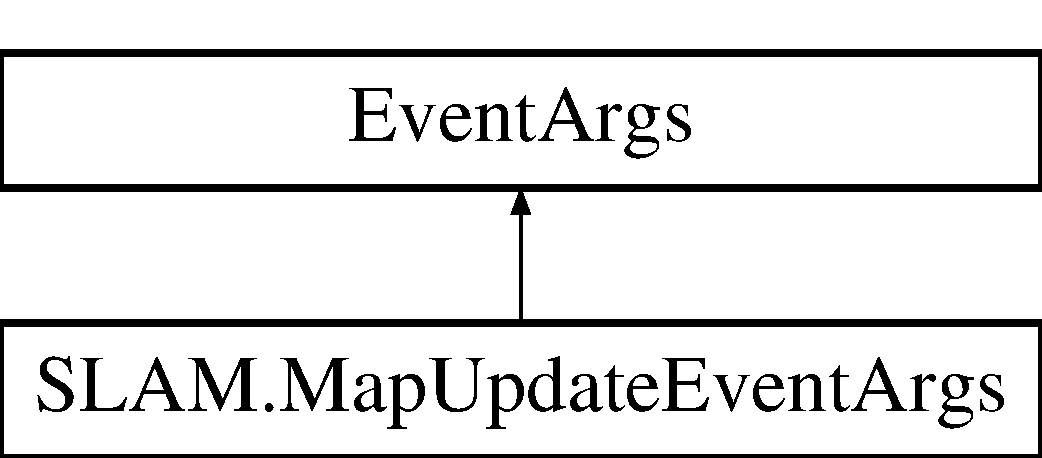
\includegraphics[height=2.000000cm]{class_s_l_a_m_1_1_map_update_event_args}
\end{center}
\end{figure}
\subsection*{Public Member Functions}
\begin{DoxyCompactItemize}
\item 
{\bf Map\-Update\-Event\-Args} ({\bf Slam\-Map} updated\-Map)
\begin{DoxyCompactList}\small\item\em Initializes a new instance of the \doxyref{S\-L\-A\-M.\-Map\-Update\-Event\-Args}{p.}{class_s_l_a_m_1_1_map_update_event_args} class. \end{DoxyCompactList}\end{DoxyCompactItemize}
\subsection*{Properties}
\begin{DoxyCompactItemize}
\item 
{\bf Slam\-Map} {\bf Map}\hspace{0.3cm}{\ttfamily  [get]}
\begin{DoxyCompactList}\small\item\em Gets the map. \end{DoxyCompactList}\end{DoxyCompactItemize}


\subsection{Detailed Description}
An event to handle any updates to the map. 



\subsection{Constructor \& Destructor Documentation}
\index{S\-L\-A\-M\-::\-Map\-Update\-Event\-Args@{S\-L\-A\-M\-::\-Map\-Update\-Event\-Args}!Map\-Update\-Event\-Args@{Map\-Update\-Event\-Args}}
\index{Map\-Update\-Event\-Args@{Map\-Update\-Event\-Args}!SLAM::MapUpdateEventArgs@{S\-L\-A\-M\-::\-Map\-Update\-Event\-Args}}
\subsubsection[{Map\-Update\-Event\-Args}]{\setlength{\rightskip}{0pt plus 5cm}S\-L\-A\-M.\-Map\-Update\-Event\-Args.\-Map\-Update\-Event\-Args (
\begin{DoxyParamCaption}
\item[{{\bf Slam\-Map}}]{updated\-Map}
\end{DoxyParamCaption}
)}\label{class_s_l_a_m_1_1_map_update_event_args_aaa7e71156ff8930089ba01b60eb35692}


Initializes a new instance of the \doxyref{S\-L\-A\-M.\-Map\-Update\-Event\-Args}{p.}{class_s_l_a_m_1_1_map_update_event_args} class. 


\begin{DoxyParams}{Parameters}
{\em updated\-Map} & Updated map.\\
\hline
\end{DoxyParams}


\subsection{Property Documentation}
\index{S\-L\-A\-M\-::\-Map\-Update\-Event\-Args@{S\-L\-A\-M\-::\-Map\-Update\-Event\-Args}!Map@{Map}}
\index{Map@{Map}!SLAM::MapUpdateEventArgs@{S\-L\-A\-M\-::\-Map\-Update\-Event\-Args}}
\subsubsection[{Map}]{\setlength{\rightskip}{0pt plus 5cm}{\bf Slam\-Map} S\-L\-A\-M.\-Map\-Update\-Event\-Args.\-Map\hspace{0.3cm}{\ttfamily [get]}}\label{class_s_l_a_m_1_1_map_update_event_args_a42780397b20c9d9ce6535a2f795ca0d3}


Gets the map. 

The map.

The documentation for this class was generated from the following file\-:\begin{DoxyCompactItemize}
\item 
S\-L\-A\-M/\-Event/{\bf Map\-Update\-Event\-Args.\-cs}\end{DoxyCompactItemize}

\section{S\-L\-A\-M.\-Map\-View Class Reference}
\label{class_s_l_a_m_1_1_map_view}\index{S\-L\-A\-M.\-Map\-View@{S\-L\-A\-M.\-Map\-View}}


Map view.  


Inheritance diagram for S\-L\-A\-M.\-Map\-View\-:\begin{figure}[H]
\begin{center}
\leavevmode
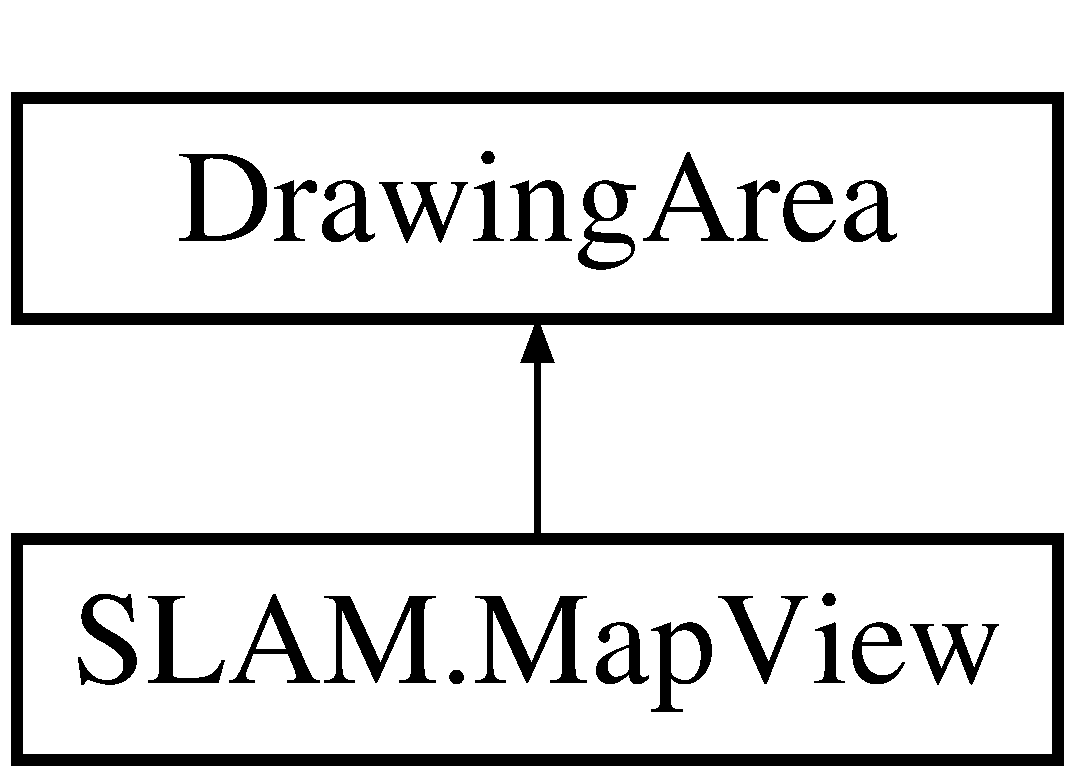
\includegraphics[height=2.000000cm]{class_s_l_a_m_1_1_map_view}
\end{center}
\end{figure}
\subsection*{Public Member Functions}
\begin{DoxyCompactItemize}
\item 
{\bf Map\-View} ({\bf Slam\-Map} map\-Model, {\bf Ekf\-Slam} Slam\-Instance)
\begin{DoxyCompactList}\small\item\em Initializes a new instance of the \doxyref{S\-L\-A\-M.\-Map\-View}{p.}{class_s_l_a_m_1_1_map_view} class. \end{DoxyCompactList}\end{DoxyCompactItemize}
\subsection*{Properties}
\begin{DoxyCompactItemize}
\item 
{\bf Slam\-Map} {\bf Map\-Model}\hspace{0.3cm}{\ttfamily  [get, set]}
\begin{DoxyCompactList}\small\item\em Gets or sets the map. \end{DoxyCompactList}\item 
{\bf Robot\-View} {\bf Robot\-View}\hspace{0.3cm}{\ttfamily  [get, set]}
\begin{DoxyCompactList}\small\item\em Gets or sets the robot view. \end{DoxyCompactList}\item 
int {\bf View\-Width}\hspace{0.3cm}{\ttfamily  [get, set]}
\begin{DoxyCompactList}\small\item\em Gets or sets the width of the view. \end{DoxyCompactList}\item 
int {\bf View\-Height}\hspace{0.3cm}{\ttfamily  [get, set]}
\begin{DoxyCompactList}\small\item\em Gets or sets the height of the view. \end{DoxyCompactList}\end{DoxyCompactItemize}


\subsection{Detailed Description}
Map view. 



\subsection{Constructor \& Destructor Documentation}
\index{S\-L\-A\-M\-::\-Map\-View@{S\-L\-A\-M\-::\-Map\-View}!Map\-View@{Map\-View}}
\index{Map\-View@{Map\-View}!SLAM::MapView@{S\-L\-A\-M\-::\-Map\-View}}
\subsubsection[{Map\-View}]{\setlength{\rightskip}{0pt plus 5cm}S\-L\-A\-M.\-Map\-View.\-Map\-View (
\begin{DoxyParamCaption}
\item[{{\bf Slam\-Map}}]{map\-Model, }
\item[{{\bf Ekf\-Slam}}]{Slam\-Instance}
\end{DoxyParamCaption}
)}\label{class_s_l_a_m_1_1_map_view_a8abf5362788639c6b021f7999ca31c0e}


Initializes a new instance of the \doxyref{S\-L\-A\-M.\-Map\-View}{p.}{class_s_l_a_m_1_1_map_view} class. 


\begin{DoxyParams}{Parameters}
{\em map\-Model} & Map model.\\
\hline
\end{DoxyParams}


\subsection{Property Documentation}
\index{S\-L\-A\-M\-::\-Map\-View@{S\-L\-A\-M\-::\-Map\-View}!Map\-Model@{Map\-Model}}
\index{Map\-Model@{Map\-Model}!SLAM::MapView@{S\-L\-A\-M\-::\-Map\-View}}
\subsubsection[{Map\-Model}]{\setlength{\rightskip}{0pt plus 5cm}{\bf Slam\-Map} S\-L\-A\-M.\-Map\-View.\-Map\-Model\hspace{0.3cm}{\ttfamily [get]}, {\ttfamily [set]}}\label{class_s_l_a_m_1_1_map_view_a6cde29763ac784e1785d13c024c0400e}


Gets or sets the map. 

The map.\index{S\-L\-A\-M\-::\-Map\-View@{S\-L\-A\-M\-::\-Map\-View}!Robot\-View@{Robot\-View}}
\index{Robot\-View@{Robot\-View}!SLAM::MapView@{S\-L\-A\-M\-::\-Map\-View}}
\subsubsection[{Robot\-View}]{\setlength{\rightskip}{0pt plus 5cm}{\bf Robot\-View} S\-L\-A\-M.\-Map\-View.\-Robot\-View\hspace{0.3cm}{\ttfamily [get]}, {\ttfamily [set]}}\label{class_s_l_a_m_1_1_map_view_a875996a502c8220bce6b18b20a0dac3c}


Gets or sets the robot view. 

The robot view.\index{S\-L\-A\-M\-::\-Map\-View@{S\-L\-A\-M\-::\-Map\-View}!View\-Height@{View\-Height}}
\index{View\-Height@{View\-Height}!SLAM::MapView@{S\-L\-A\-M\-::\-Map\-View}}
\subsubsection[{View\-Height}]{\setlength{\rightskip}{0pt plus 5cm}int S\-L\-A\-M.\-Map\-View.\-View\-Height\hspace{0.3cm}{\ttfamily [get]}, {\ttfamily [set]}}\label{class_s_l_a_m_1_1_map_view_adbe91d7463c5e359ac81cd09bc663be3}


Gets or sets the height of the view. 

The height of the view.\index{S\-L\-A\-M\-::\-Map\-View@{S\-L\-A\-M\-::\-Map\-View}!View\-Width@{View\-Width}}
\index{View\-Width@{View\-Width}!SLAM::MapView@{S\-L\-A\-M\-::\-Map\-View}}
\subsubsection[{View\-Width}]{\setlength{\rightskip}{0pt plus 5cm}int S\-L\-A\-M.\-Map\-View.\-View\-Width\hspace{0.3cm}{\ttfamily [get]}, {\ttfamily [set]}}\label{class_s_l_a_m_1_1_map_view_aa8bea59e255e6a0a60f5cdb069729abd}


Gets or sets the width of the view. 

The width of the view.

The documentation for this class was generated from the following file\-:\begin{DoxyCompactItemize}
\item 
S\-L\-A\-M/\-View/{\bf Map\-View.\-cs}\end{DoxyCompactItemize}

\section{S\-L\-A\-M.\-Map\-Window Class Reference}
\label{class_s_l_a_m_1_1_map_window}\index{S\-L\-A\-M.\-Map\-Window@{S\-L\-A\-M.\-Map\-Window}}


Map window.  


Inheritance diagram for S\-L\-A\-M.\-Map\-Window\-:\begin{figure}[H]
\begin{center}
\leavevmode
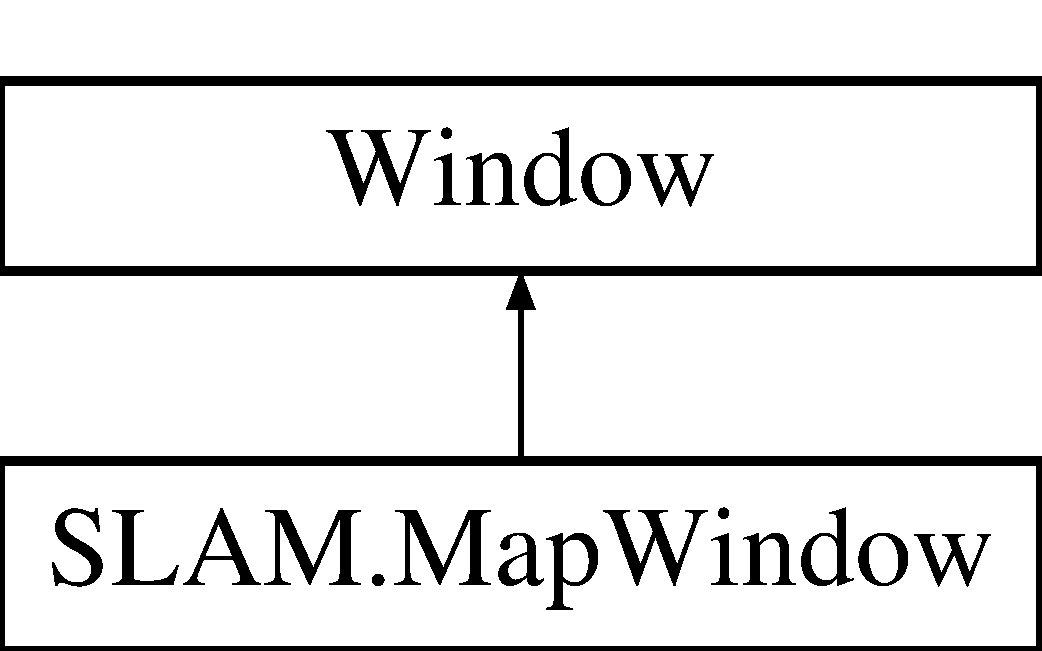
\includegraphics[height=2.000000cm]{class_s_l_a_m_1_1_map_window}
\end{center}
\end{figure}
\subsection*{Public Member Functions}
\begin{DoxyCompactItemize}
\item 
{\bf Map\-Window} ({\bf Map\-View} map\-View)
\begin{DoxyCompactList}\small\item\em Initializes a new instance of the \doxyref{S\-L\-A\-M.\-Map\-Window}{p.}{class_s_l_a_m_1_1_map_window} class. \end{DoxyCompactList}\end{DoxyCompactItemize}


\subsection{Detailed Description}
Map window. 



\subsection{Constructor \& Destructor Documentation}
\index{S\-L\-A\-M\-::\-Map\-Window@{S\-L\-A\-M\-::\-Map\-Window}!Map\-Window@{Map\-Window}}
\index{Map\-Window@{Map\-Window}!SLAM::MapWindow@{S\-L\-A\-M\-::\-Map\-Window}}
\subsubsection[{Map\-Window}]{\setlength{\rightskip}{0pt plus 5cm}S\-L\-A\-M.\-Map\-Window.\-Map\-Window (
\begin{DoxyParamCaption}
\item[{{\bf Map\-View}}]{map\-View}
\end{DoxyParamCaption}
)}\label{class_s_l_a_m_1_1_map_window_a29b92ae6683eed26ed5409cda955652a}


Initializes a new instance of the \doxyref{S\-L\-A\-M.\-Map\-Window}{p.}{class_s_l_a_m_1_1_map_window} class. 


\begin{DoxyParams}{Parameters}
{\em map\-View} & Map view contained in this window.\\
\hline
\end{DoxyParams}


The documentation for this class was generated from the following file\-:\begin{DoxyCompactItemize}
\item 
S\-L\-A\-M/\-View/{\bf Map\-Window.\-cs}\end{DoxyCompactItemize}

\section{S\-L\-A\-M.\-Path\-View Class Reference}
\label{class_s_l_a_m_1_1_path_view}\index{S\-L\-A\-M.\-Path\-View@{S\-L\-A\-M.\-Path\-View}}


Path view. Keeps Track of where the robot has been visually on the map  


\subsection*{Public Member Functions}
\begin{DoxyCompactItemize}
\item 
{\bf Path\-View} ({\bf Robot} robot\-Model)
\begin{DoxyCompactList}\small\item\em Initializes a new instance of the \doxyref{S\-L\-A\-M.\-Path\-View}{p.}{class_s_l_a_m_1_1_path_view} class. \end{DoxyCompactList}\item 
void {\bf Draw} (Cairo.\-Context cairo\-Context, int center\-X, int center\-Y, double scale)
\begin{DoxyCompactList}\small\item\em Draw the specified cairo\-Context, center\-X, center\-Y and scale. \end{DoxyCompactList}\end{DoxyCompactItemize}


\subsection{Detailed Description}
Path view. Keeps Track of where the robot has been visually on the map 



\subsection{Constructor \& Destructor Documentation}
\index{S\-L\-A\-M\-::\-Path\-View@{S\-L\-A\-M\-::\-Path\-View}!Path\-View@{Path\-View}}
\index{Path\-View@{Path\-View}!SLAM::PathView@{S\-L\-A\-M\-::\-Path\-View}}
\subsubsection[{Path\-View}]{\setlength{\rightskip}{0pt plus 5cm}S\-L\-A\-M.\-Path\-View.\-Path\-View (
\begin{DoxyParamCaption}
\item[{{\bf Robot}}]{robot\-Model}
\end{DoxyParamCaption}
)}\label{class_s_l_a_m_1_1_path_view_a0b053bd95d0547e8047cafc29432613a}


Initializes a new instance of the \doxyref{S\-L\-A\-M.\-Path\-View}{p.}{class_s_l_a_m_1_1_path_view} class. 


\begin{DoxyParams}{Parameters}
{\em robot\-Model} & The instance oif the robot that will be followed.\\
\hline
\end{DoxyParams}


\subsection{Member Function Documentation}
\index{S\-L\-A\-M\-::\-Path\-View@{S\-L\-A\-M\-::\-Path\-View}!Draw@{Draw}}
\index{Draw@{Draw}!SLAM::PathView@{S\-L\-A\-M\-::\-Path\-View}}
\subsubsection[{Draw}]{\setlength{\rightskip}{0pt plus 5cm}void S\-L\-A\-M.\-Path\-View.\-Draw (
\begin{DoxyParamCaption}
\item[{Cairo.\-Context}]{cairo\-Context, }
\item[{int}]{center\-X, }
\item[{int}]{center\-Y, }
\item[{double}]{scale}
\end{DoxyParamCaption}
)}\label{class_s_l_a_m_1_1_path_view_a7920979987b2ca4f364a665eded7569d}


Draw the specified cairo\-Context, center\-X, center\-Y and scale. 


\begin{DoxyParams}{Parameters}
{\em cairo\-Context} & Cairo context.\\
\hline
{\em center\-X} & Center x.\\
\hline
{\em center\-Y} & Center y.\\
\hline
{\em scale} & Scale.\\
\hline
\end{DoxyParams}


The documentation for this class was generated from the following file\-:\begin{DoxyCompactItemize}
\item 
S\-L\-A\-M/\-View/{\bf Path\-View.\-cs}\end{DoxyCompactItemize}

\section{S\-L\-A\-M.\-Robot Class Reference}
\label{class_s_l_a_m_1_1_robot}\index{S\-L\-A\-M.\-Robot@{S\-L\-A\-M.\-Robot}}


Contains the exploration robot model as part of the Model-\/\-View-\/\-Controller (M\-V\-C) design pattern. This class does not contain any view specific code instead it acts as a state model for the robot recording its current x and y position, rotation, and state.  


\subsection*{Public Member Functions}
\begin{DoxyCompactItemize}
\item 
{\bf Robot} ()
\begin{DoxyCompactList}\small\item\em Initializes a new instance of the \doxyref{S\-L\-A\-M.\-Robot}{p.}{class_s_l_a_m_1_1_robot} class with the default settings for the Pirate robot platform. \end{DoxyCompactList}\item 
{\bf Robot} (double x\-Position, double y\-Position, double current\-Rotation, {\bf Robot\-State} current\-State, double robot\-Width, double robot\-Height, double cpi)
\begin{DoxyCompactList}\small\item\em Initializes a new instance of the \doxyref{S\-L\-A\-M.\-Robot}{p.}{class_s_l_a_m_1_1_robot} class. \end{DoxyCompactList}\item 
void {\bf Go\-Foward} ()
\item 
void {\bf Go\-Backward} ()
\item 
void {\bf Rotate\-Left} ()
\item 
void {\bf Rotate\-Right} ()
\item 
void {\bf Halt} ()
\item 
void {\bf Scan} ()
\item 
void {\bf Update\-Odometry} (Odometry\-Update\-Event\-Args e)
\begin{DoxyCompactList}\small\item\em Updates the odometry. \end{DoxyCompactList}\end{DoxyCompactItemize}
\subsection*{Protected Member Functions}
\begin{DoxyCompactItemize}
\item 
virtual void {\bf On\-Robot\-Update} ({\bf Robot\-Update\-Event\-Args} e)
\begin{DoxyCompactList}\small\item\em Raises the robot update event. \end{DoxyCompactList}\end{DoxyCompactItemize}
\subsection*{Properties}
\begin{DoxyCompactItemize}
\item 
double {\bf X}\hspace{0.3cm}{\ttfamily  [get, set]}
\begin{DoxyCompactList}\small\item\em Gets or sets the x position of the robot in its environment. \end{DoxyCompactList}\item 
double {\bf Y}\hspace{0.3cm}{\ttfamily  [get, set]}
\begin{DoxyCompactList}\small\item\em Gets or sets the y position of the robot in its environment. \end{DoxyCompactList}\item 
double {\bf Heading}\hspace{0.3cm}{\ttfamily  [get, set]}
\begin{DoxyCompactList}\small\item\em Gets or sets the rotation of the robot in radians. \end{DoxyCompactList}\item 
{\bf Robot\-State} {\bf State}\hspace{0.3cm}{\ttfamily  [get, set]}
\begin{DoxyCompactList}\small\item\em Gets or sets the state of the robot \doxyref{S\-L\-A\-M.\-Robot\-State}{p.}{namespace_s_l_a_m_af423bd61f5623a682e45a0d9430cf946}. \end{DoxyCompactList}\item 
double {\bf Width}\hspace{0.3cm}{\ttfamily  [get]}
\begin{DoxyCompactList}\small\item\em Gets the width. \end{DoxyCompactList}\item 
double {\bf Height}\hspace{0.3cm}{\ttfamily  [get]}
\begin{DoxyCompactList}\small\item\em Gets the height. \end{DoxyCompactList}\item 
double[$\,$] {\bf Position}\hspace{0.3cm}{\ttfamily  [get]}
\begin{DoxyCompactList}\small\item\em Gets the robot's position as an array containing x, y, and rotation. \end{DoxyCompactList}\item 
double {\bf Cpi}\hspace{0.3cm}{\ttfamily  [get, set]}
\begin{DoxyCompactList}\small\item\em Gets or sets the cpi of the mouse sensor. \end{DoxyCompactList}\item 
List$<$ double[$\,$]$>$ {\bf Path\-Point\-List}\hspace{0.3cm}{\ttfamily  [get, set]}
\begin{DoxyCompactList}\small\item\em Gets or sets the x position of the robot in its environment. \end{DoxyCompactList}\end{DoxyCompactItemize}
\subsection*{Events}
\begin{DoxyCompactItemize}
\item 
Event\-Handler\\*
$<$ {\bf Robot\-Update\-Event\-Args} $>$ {\bf Robot\-Updated}
\end{DoxyCompactItemize}


\subsection{Detailed Description}
Contains the exploration robot model as part of the Model-\/\-View-\/\-Controller (M\-V\-C) design pattern. This class does not contain any view specific code instead it acts as a state model for the robot recording its current x and y position, rotation, and state. 

Whenever there is a change to the robot a {\ttfamily \doxyref{Robot\-Update\-Event\-Args}{p.}{class_s_l_a_m_1_1_robot_update_event_args}} is raised to inform any observers that there has been an update to the robot's state. 

\subsection{Constructor \& Destructor Documentation}
\index{S\-L\-A\-M\-::\-Robot@{S\-L\-A\-M\-::\-Robot}!Robot@{Robot}}
\index{Robot@{Robot}!SLAM::Robot@{S\-L\-A\-M\-::\-Robot}}
\subsubsection[{Robot}]{\setlength{\rightskip}{0pt plus 5cm}S\-L\-A\-M.\-Robot.\-Robot (
\begin{DoxyParamCaption}
{}
\end{DoxyParamCaption}
)}\label{class_s_l_a_m_1_1_robot_a3c15a152318e456a7cadfdbe29813764}


Initializes a new instance of the \doxyref{S\-L\-A\-M.\-Robot}{p.}{class_s_l_a_m_1_1_robot} class with the default settings for the Pirate robot platform. 

\index{S\-L\-A\-M\-::\-Robot@{S\-L\-A\-M\-::\-Robot}!Robot@{Robot}}
\index{Robot@{Robot}!SLAM::Robot@{S\-L\-A\-M\-::\-Robot}}
\subsubsection[{Robot}]{\setlength{\rightskip}{0pt plus 5cm}S\-L\-A\-M.\-Robot.\-Robot (
\begin{DoxyParamCaption}
\item[{double}]{x\-Position, }
\item[{double}]{y\-Position, }
\item[{double}]{current\-Rotation, }
\item[{{\bf Robot\-State}}]{current\-State, }
\item[{double}]{robot\-Width, }
\item[{double}]{robot\-Height, }
\item[{double}]{cpi}
\end{DoxyParamCaption}
)}\label{class_s_l_a_m_1_1_robot_aca6e01be616c4c8dcc669f8d4e8c9a2f}


Initializes a new instance of the \doxyref{S\-L\-A\-M.\-Robot}{p.}{class_s_l_a_m_1_1_robot} class. 


\begin{DoxyParams}{Parameters}
{\em x\-Position} & X position in meters.\\
\hline
{\em y\-Position} & Y position in meters.\\
\hline
{\em current\-Rotation} & Current rotation in radians.\\
\hline
{\em current\-State} & Current state \doxyref{S\-L\-A\-M.\-Robot\-State}{p.}{namespace_s_l_a_m_af423bd61f5623a682e45a0d9430cf946}.\\
\hline
{\em robot\-Width} & \doxyref{Robot}{p.}{class_s_l_a_m_1_1_robot} width in meters.\\
\hline
{\em robot\-Height} & \doxyref{Robot}{p.}{class_s_l_a_m_1_1_robot} height in meters.\\
\hline
\end{DoxyParams}


\subsection{Member Function Documentation}
\index{S\-L\-A\-M\-::\-Robot@{S\-L\-A\-M\-::\-Robot}!Go\-Backward@{Go\-Backward}}
\index{Go\-Backward@{Go\-Backward}!SLAM::Robot@{S\-L\-A\-M\-::\-Robot}}
\subsubsection[{Go\-Backward}]{\setlength{\rightskip}{0pt plus 5cm}void S\-L\-A\-M.\-Robot.\-Go\-Backward (
\begin{DoxyParamCaption}
{}
\end{DoxyParamCaption}
)}\label{class_s_l_a_m_1_1_robot_ac6b53f4da55b7bae6a1df213c848c01e}
\index{S\-L\-A\-M\-::\-Robot@{S\-L\-A\-M\-::\-Robot}!Go\-Foward@{Go\-Foward}}
\index{Go\-Foward@{Go\-Foward}!SLAM::Robot@{S\-L\-A\-M\-::\-Robot}}
\subsubsection[{Go\-Foward}]{\setlength{\rightskip}{0pt plus 5cm}void S\-L\-A\-M.\-Robot.\-Go\-Foward (
\begin{DoxyParamCaption}
{}
\end{DoxyParamCaption}
)}\label{class_s_l_a_m_1_1_robot_a779c298c447a967cef34a12cf7fbea0b}
\index{S\-L\-A\-M\-::\-Robot@{S\-L\-A\-M\-::\-Robot}!Halt@{Halt}}
\index{Halt@{Halt}!SLAM::Robot@{S\-L\-A\-M\-::\-Robot}}
\subsubsection[{Halt}]{\setlength{\rightskip}{0pt plus 5cm}void S\-L\-A\-M.\-Robot.\-Halt (
\begin{DoxyParamCaption}
{}
\end{DoxyParamCaption}
)}\label{class_s_l_a_m_1_1_robot_a0c2a5aaa45c36522f2f35b14aa7c9d87}
\index{S\-L\-A\-M\-::\-Robot@{S\-L\-A\-M\-::\-Robot}!On\-Robot\-Update@{On\-Robot\-Update}}
\index{On\-Robot\-Update@{On\-Robot\-Update}!SLAM::Robot@{S\-L\-A\-M\-::\-Robot}}
\subsubsection[{On\-Robot\-Update}]{\setlength{\rightskip}{0pt plus 5cm}virtual void S\-L\-A\-M.\-Robot.\-On\-Robot\-Update (
\begin{DoxyParamCaption}
\item[{{\bf Robot\-Update\-Event\-Args}}]{e}
\end{DoxyParamCaption}
)\hspace{0.3cm}{\ttfamily [protected]}, {\ttfamily [virtual]}}\label{class_s_l_a_m_1_1_robot_aa2298cbc031eddc7407141c85df0f696}


Raises the robot update event. 


\begin{DoxyParams}{Parameters}
{\em e} & E.\\
\hline
\end{DoxyParams}
\index{S\-L\-A\-M\-::\-Robot@{S\-L\-A\-M\-::\-Robot}!Rotate\-Left@{Rotate\-Left}}
\index{Rotate\-Left@{Rotate\-Left}!SLAM::Robot@{S\-L\-A\-M\-::\-Robot}}
\subsubsection[{Rotate\-Left}]{\setlength{\rightskip}{0pt plus 5cm}void S\-L\-A\-M.\-Robot.\-Rotate\-Left (
\begin{DoxyParamCaption}
{}
\end{DoxyParamCaption}
)}\label{class_s_l_a_m_1_1_robot_aefc7b6664cecc2ad987367174bebc28c}
\index{S\-L\-A\-M\-::\-Robot@{S\-L\-A\-M\-::\-Robot}!Rotate\-Right@{Rotate\-Right}}
\index{Rotate\-Right@{Rotate\-Right}!SLAM::Robot@{S\-L\-A\-M\-::\-Robot}}
\subsubsection[{Rotate\-Right}]{\setlength{\rightskip}{0pt plus 5cm}void S\-L\-A\-M.\-Robot.\-Rotate\-Right (
\begin{DoxyParamCaption}
{}
\end{DoxyParamCaption}
)}\label{class_s_l_a_m_1_1_robot_a0c94d92a5bba9e2e8a324f6c8e0d3f84}
\index{S\-L\-A\-M\-::\-Robot@{S\-L\-A\-M\-::\-Robot}!Scan@{Scan}}
\index{Scan@{Scan}!SLAM::Robot@{S\-L\-A\-M\-::\-Robot}}
\subsubsection[{Scan}]{\setlength{\rightskip}{0pt plus 5cm}void S\-L\-A\-M.\-Robot.\-Scan (
\begin{DoxyParamCaption}
{}
\end{DoxyParamCaption}
)}\label{class_s_l_a_m_1_1_robot_ae41d52d452d35705f619705d9d5f1bb0}
\index{S\-L\-A\-M\-::\-Robot@{S\-L\-A\-M\-::\-Robot}!Update\-Odometry@{Update\-Odometry}}
\index{Update\-Odometry@{Update\-Odometry}!SLAM::Robot@{S\-L\-A\-M\-::\-Robot}}
\subsubsection[{Update\-Odometry}]{\setlength{\rightskip}{0pt plus 5cm}void S\-L\-A\-M.\-Robot.\-Update\-Odometry (
\begin{DoxyParamCaption}
\item[{Odometry\-Update\-Event\-Args}]{e}
\end{DoxyParamCaption}
)}\label{class_s_l_a_m_1_1_robot_a2ddc0e9dacffa9dac975525d1ab8ec5f}


Updates the odometry. 


\begin{DoxyParams}{Parameters}
{\em e} & E.\\
\hline
\end{DoxyParams}


\subsection{Property Documentation}
\index{S\-L\-A\-M\-::\-Robot@{S\-L\-A\-M\-::\-Robot}!Cpi@{Cpi}}
\index{Cpi@{Cpi}!SLAM::Robot@{S\-L\-A\-M\-::\-Robot}}
\subsubsection[{Cpi}]{\setlength{\rightskip}{0pt plus 5cm}double S\-L\-A\-M.\-Robot.\-Cpi\hspace{0.3cm}{\ttfamily [get]}, {\ttfamily [set]}}\label{class_s_l_a_m_1_1_robot_a02c042efe44ab418544f1258af6c5bc4}


Gets or sets the cpi of the mouse sensor. 

The cpi resolution.\index{S\-L\-A\-M\-::\-Robot@{S\-L\-A\-M\-::\-Robot}!Heading@{Heading}}
\index{Heading@{Heading}!SLAM::Robot@{S\-L\-A\-M\-::\-Robot}}
\subsubsection[{Heading}]{\setlength{\rightskip}{0pt plus 5cm}double S\-L\-A\-M.\-Robot.\-Heading\hspace{0.3cm}{\ttfamily [get]}, {\ttfamily [set]}}\label{class_s_l_a_m_1_1_robot_a08d9e43c5ffb45a413b9850a0c1b3200}


Gets or sets the rotation of the robot in radians. 

The new rotation in radians.\index{S\-L\-A\-M\-::\-Robot@{S\-L\-A\-M\-::\-Robot}!Height@{Height}}
\index{Height@{Height}!SLAM::Robot@{S\-L\-A\-M\-::\-Robot}}
\subsubsection[{Height}]{\setlength{\rightskip}{0pt plus 5cm}double S\-L\-A\-M.\-Robot.\-Height\hspace{0.3cm}{\ttfamily [get]}}\label{class_s_l_a_m_1_1_robot_ad26ede2b897b030613c5591346343ef7}


Gets the height. 

The height of the robot in meters.\index{S\-L\-A\-M\-::\-Robot@{S\-L\-A\-M\-::\-Robot}!Path\-Point\-List@{Path\-Point\-List}}
\index{Path\-Point\-List@{Path\-Point\-List}!SLAM::Robot@{S\-L\-A\-M\-::\-Robot}}
\subsubsection[{Path\-Point\-List}]{\setlength{\rightskip}{0pt plus 5cm}List$<$double[$\,$]$>$ S\-L\-A\-M.\-Robot.\-Path\-Point\-List\hspace{0.3cm}{\ttfamily [get]}, {\ttfamily [set]}}\label{class_s_l_a_m_1_1_robot_a6376d1570c96ecca55cbccb11dbbd6f7}


Gets or sets the x position of the robot in its environment. 

The new x position in meters.\index{S\-L\-A\-M\-::\-Robot@{S\-L\-A\-M\-::\-Robot}!Position@{Position}}
\index{Position@{Position}!SLAM::Robot@{S\-L\-A\-M\-::\-Robot}}
\subsubsection[{Position}]{\setlength{\rightskip}{0pt plus 5cm}double [$\,$] S\-L\-A\-M.\-Robot.\-Position\hspace{0.3cm}{\ttfamily [get]}}\label{class_s_l_a_m_1_1_robot_a997078dbe427376750c5a145ad0123fd}


Gets the robot's position as an array containing x, y, and rotation. 

The position as an array.\index{S\-L\-A\-M\-::\-Robot@{S\-L\-A\-M\-::\-Robot}!State@{State}}
\index{State@{State}!SLAM::Robot@{S\-L\-A\-M\-::\-Robot}}
\subsubsection[{State}]{\setlength{\rightskip}{0pt plus 5cm}{\bf Robot\-State} S\-L\-A\-M.\-Robot.\-State\hspace{0.3cm}{\ttfamily [get]}, {\ttfamily [set]}}\label{class_s_l_a_m_1_1_robot_a1d29b1831bf203faec06a9e59dd37255}


Gets or sets the state of the robot \doxyref{S\-L\-A\-M.\-Robot\-State}{p.}{namespace_s_l_a_m_af423bd61f5623a682e45a0d9430cf946}. 

The new state of the robot.\index{S\-L\-A\-M\-::\-Robot@{S\-L\-A\-M\-::\-Robot}!Width@{Width}}
\index{Width@{Width}!SLAM::Robot@{S\-L\-A\-M\-::\-Robot}}
\subsubsection[{Width}]{\setlength{\rightskip}{0pt plus 5cm}double S\-L\-A\-M.\-Robot.\-Width\hspace{0.3cm}{\ttfamily [get]}}\label{class_s_l_a_m_1_1_robot_ad606a04d3b6f349f9e9a93f613aa40e2}


Gets the width. 

The width of the robot in meters.\index{S\-L\-A\-M\-::\-Robot@{S\-L\-A\-M\-::\-Robot}!X@{X}}
\index{X@{X}!SLAM::Robot@{S\-L\-A\-M\-::\-Robot}}
\subsubsection[{X}]{\setlength{\rightskip}{0pt plus 5cm}double S\-L\-A\-M.\-Robot.\-X\hspace{0.3cm}{\ttfamily [get]}, {\ttfamily [set]}}\label{class_s_l_a_m_1_1_robot_a65a2fb5de14325f68d83b36c7751bd96}


Gets or sets the x position of the robot in its environment. 

The new x position in meters.\index{S\-L\-A\-M\-::\-Robot@{S\-L\-A\-M\-::\-Robot}!Y@{Y}}
\index{Y@{Y}!SLAM::Robot@{S\-L\-A\-M\-::\-Robot}}
\subsubsection[{Y}]{\setlength{\rightskip}{0pt plus 5cm}double S\-L\-A\-M.\-Robot.\-Y\hspace{0.3cm}{\ttfamily [get]}, {\ttfamily [set]}}\label{class_s_l_a_m_1_1_robot_a5bf2a77534812a416dcbf90651966e4e}


Gets or sets the y position of the robot in its environment. 

The new y position in meters.

\subsection{Event Documentation}
\index{S\-L\-A\-M\-::\-Robot@{S\-L\-A\-M\-::\-Robot}!Robot\-Updated@{Robot\-Updated}}
\index{Robot\-Updated@{Robot\-Updated}!SLAM::Robot@{S\-L\-A\-M\-::\-Robot}}
\subsubsection[{Robot\-Updated}]{\setlength{\rightskip}{0pt plus 5cm}Event\-Handler$<${\bf Robot\-Update\-Event\-Args}$>$ S\-L\-A\-M.\-Robot.\-Robot\-Updated}\label{class_s_l_a_m_1_1_robot_a27f408587eafb528ab62dd3568293e37}


The documentation for this class was generated from the following file\-:\begin{DoxyCompactItemize}
\item 
S\-L\-A\-M/\-Model/{\bf Robot.\-cs}\end{DoxyCompactItemize}

\section{S\-L\-A\-M.\-Robot\-Update\-Event\-Args Class Reference}
\label{class_s_l_a_m_1_1_robot_update_event_args}\index{S\-L\-A\-M.\-Robot\-Update\-Event\-Args@{S\-L\-A\-M.\-Robot\-Update\-Event\-Args}}


An event to handle any updates to the robot.  


Inheritance diagram for S\-L\-A\-M.\-Robot\-Update\-Event\-Args\-:\begin{figure}[H]
\begin{center}
\leavevmode
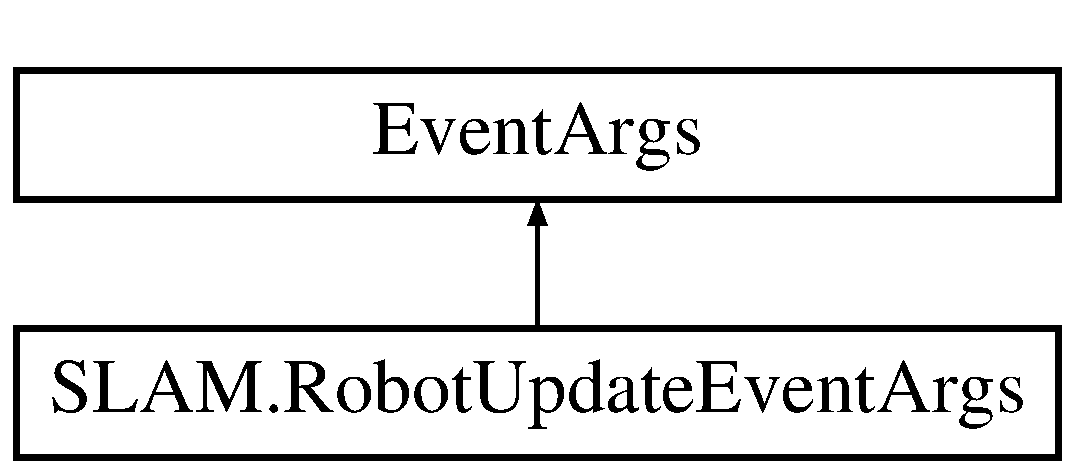
\includegraphics[height=2.000000cm]{class_s_l_a_m_1_1_robot_update_event_args}
\end{center}
\end{figure}
\subsection*{Public Member Functions}
\begin{DoxyCompactItemize}
\item 
{\bf Robot\-Update\-Event\-Args} ({\bf Robot} updated\-Robot)
\item 
override string {\bf To\-String} ()
\end{DoxyCompactItemize}
\subsection*{Properties}
\begin{DoxyCompactItemize}
\item 
{\bf Robot} {\bf Robot}\hspace{0.3cm}{\ttfamily  [get]}
\end{DoxyCompactItemize}


\subsection{Detailed Description}
An event to handle any updates to the robot. 



\subsection{Constructor \& Destructor Documentation}
\index{S\-L\-A\-M\-::\-Robot\-Update\-Event\-Args@{S\-L\-A\-M\-::\-Robot\-Update\-Event\-Args}!Robot\-Update\-Event\-Args@{Robot\-Update\-Event\-Args}}
\index{Robot\-Update\-Event\-Args@{Robot\-Update\-Event\-Args}!SLAM::RobotUpdateEventArgs@{S\-L\-A\-M\-::\-Robot\-Update\-Event\-Args}}
\subsubsection[{Robot\-Update\-Event\-Args}]{\setlength{\rightskip}{0pt plus 5cm}S\-L\-A\-M.\-Robot\-Update\-Event\-Args.\-Robot\-Update\-Event\-Args (
\begin{DoxyParamCaption}
\item[{{\bf Robot}}]{updated\-Robot}
\end{DoxyParamCaption}
)}\label{class_s_l_a_m_1_1_robot_update_event_args_a0c21c4d867bc241ab66a7801b6eec672}


\subsection{Member Function Documentation}
\index{S\-L\-A\-M\-::\-Robot\-Update\-Event\-Args@{S\-L\-A\-M\-::\-Robot\-Update\-Event\-Args}!To\-String@{To\-String}}
\index{To\-String@{To\-String}!SLAM::RobotUpdateEventArgs@{S\-L\-A\-M\-::\-Robot\-Update\-Event\-Args}}
\subsubsection[{To\-String}]{\setlength{\rightskip}{0pt plus 5cm}override string S\-L\-A\-M.\-Robot\-Update\-Event\-Args.\-To\-String (
\begin{DoxyParamCaption}
{}
\end{DoxyParamCaption}
)}\label{class_s_l_a_m_1_1_robot_update_event_args_a625a383289ac727f3acd86741866c310}


\subsection{Property Documentation}
\index{S\-L\-A\-M\-::\-Robot\-Update\-Event\-Args@{S\-L\-A\-M\-::\-Robot\-Update\-Event\-Args}!Robot@{Robot}}
\index{Robot@{Robot}!SLAM::RobotUpdateEventArgs@{S\-L\-A\-M\-::\-Robot\-Update\-Event\-Args}}
\subsubsection[{Robot}]{\setlength{\rightskip}{0pt plus 5cm}{\bf Robot} S\-L\-A\-M.\-Robot\-Update\-Event\-Args.\-Robot\hspace{0.3cm}{\ttfamily [get]}}\label{class_s_l_a_m_1_1_robot_update_event_args_aa0313cb7812dd88ea30deb47b6d5af39}


The documentation for this class was generated from the following file\-:\begin{DoxyCompactItemize}
\item 
S\-L\-A\-M/\-Event/{\bf Robot\-Update\-Event\-Args.\-cs}\end{DoxyCompactItemize}

\section{S\-L\-A\-M.\-Robot\-View Class Reference}
\label{class_s_l_a_m_1_1_robot_view}\index{S\-L\-A\-M.\-Robot\-View@{S\-L\-A\-M.\-Robot\-View}}


\doxyref{Robot}{p.}{class_s_l_a_m_1_1_robot} view.  


\subsection*{Public Member Functions}
\begin{DoxyCompactItemize}
\item 
{\bf Robot\-View} ({\bf Robot} robot\-Model)
\begin{DoxyCompactList}\small\item\em Initializes a new instance of the \doxyref{S\-L\-A\-M.\-Robot\-View}{p.}{class_s_l_a_m_1_1_robot_view} class. \end{DoxyCompactList}\item 
void {\bf Draw} (Cairo.\-Context cairo\-Context, int center\-X, int center\-Y, double scale)
\begin{DoxyCompactList}\small\item\em Draw the robot taking into account the center x and y position of the map which will be different from the true center x and y positions on the drawing context. This method will result in a red wheeled robot with black tyres being drawn at the robots location on the map. \end{DoxyCompactList}\end{DoxyCompactItemize}
\subsection*{Properties}
\begin{DoxyCompactItemize}
\item 
{\bf Robot} {\bf Robot}\hspace{0.3cm}{\ttfamily  [get]}
\end{DoxyCompactItemize}


\subsection{Detailed Description}
\doxyref{Robot}{p.}{class_s_l_a_m_1_1_robot} view. 



\subsection{Constructor \& Destructor Documentation}
\index{S\-L\-A\-M\-::\-Robot\-View@{S\-L\-A\-M\-::\-Robot\-View}!Robot\-View@{Robot\-View}}
\index{Robot\-View@{Robot\-View}!SLAM::RobotView@{S\-L\-A\-M\-::\-Robot\-View}}
\subsubsection[{Robot\-View}]{\setlength{\rightskip}{0pt plus 5cm}S\-L\-A\-M.\-Robot\-View.\-Robot\-View (
\begin{DoxyParamCaption}
\item[{{\bf Robot}}]{robot\-Model}
\end{DoxyParamCaption}
)}\label{class_s_l_a_m_1_1_robot_view_a953679008e209198a94274612300486f}


Initializes a new instance of the \doxyref{S\-L\-A\-M.\-Robot\-View}{p.}{class_s_l_a_m_1_1_robot_view} class. 


\begin{DoxyParams}{Parameters}
{\em robot\-Model} & \doxyref{Robot}{p.}{class_s_l_a_m_1_1_robot} model that this view represents.\\
\hline
\end{DoxyParams}


\subsection{Member Function Documentation}
\index{S\-L\-A\-M\-::\-Robot\-View@{S\-L\-A\-M\-::\-Robot\-View}!Draw@{Draw}}
\index{Draw@{Draw}!SLAM::RobotView@{S\-L\-A\-M\-::\-Robot\-View}}
\subsubsection[{Draw}]{\setlength{\rightskip}{0pt plus 5cm}void S\-L\-A\-M.\-Robot\-View.\-Draw (
\begin{DoxyParamCaption}
\item[{Cairo.\-Context}]{cairo\-Context, }
\item[{int}]{center\-X, }
\item[{int}]{center\-Y, }
\item[{double}]{scale}
\end{DoxyParamCaption}
)}\label{class_s_l_a_m_1_1_robot_view_a83c9cda0b93b15cc76b1f3f6a4a45add}


Draw the robot taking into account the center x and y position of the map which will be different from the true center x and y positions on the drawing context. This method will result in a red wheeled robot with black tyres being drawn at the robots location on the map. 

The scale value is currently unused but it could be useful if the map was scaled in some way for example a mini-\/map may be 10 times smaller than the original results in 1\-:10 scale robot. 


\begin{DoxyParams}{Parameters}
{\em cairo\-Context} & Cairo context to draw to (assuming a map).\\
\hline
{\em center\-X} & Center x position of map to draw onto.\\
\hline
{\em center\-Y} & Center y position of map to draw onto.\\
\hline
{\em scale} & Scale currently unused.\\
\hline
\end{DoxyParams}


\subsection{Property Documentation}
\index{S\-L\-A\-M\-::\-Robot\-View@{S\-L\-A\-M\-::\-Robot\-View}!Robot@{Robot}}
\index{Robot@{Robot}!SLAM::RobotView@{S\-L\-A\-M\-::\-Robot\-View}}
\subsubsection[{Robot}]{\setlength{\rightskip}{0pt plus 5cm}{\bf Robot} S\-L\-A\-M.\-Robot\-View.\-Robot\hspace{0.3cm}{\ttfamily [get]}}\label{class_s_l_a_m_1_1_robot_view_a31232262f149bda4b3233b4ca105d764}


The documentation for this class was generated from the following file\-:\begin{DoxyCompactItemize}
\item 
S\-L\-A\-M/\-View/{\bf Robot\-View.\-cs}\end{DoxyCompactItemize}

\section{S\-L\-A\-M.\-S\-L\-A\-M Class Reference}
\label{class_s_l_a_m_1_1_s_l_a_m}\index{S\-L\-A\-M.\-S\-L\-A\-M@{S\-L\-A\-M.\-S\-L\-A\-M}}
\subsection*{Public Member Functions}
\begin{DoxyCompactItemize}
\item 
{\bf S\-L\-A\-M} ()
\item 
void {\bf Start} ()
\end{DoxyCompactItemize}
\subsection*{Static Public Member Functions}
\begin{DoxyCompactItemize}
\item 
static void {\bf Main} (String[$\,$] args)
\end{DoxyCompactItemize}


\subsection{Constructor \& Destructor Documentation}
\index{S\-L\-A\-M\-::\-S\-L\-A\-M@{S\-L\-A\-M\-::\-S\-L\-A\-M}!S\-L\-A\-M@{S\-L\-A\-M}}
\index{S\-L\-A\-M@{S\-L\-A\-M}!SLAM::SLAM@{S\-L\-A\-M\-::\-S\-L\-A\-M}}
\subsubsection[{S\-L\-A\-M}]{\setlength{\rightskip}{0pt plus 5cm}S\-L\-A\-M.\-S\-L\-A\-M.\-S\-L\-A\-M (
\begin{DoxyParamCaption}
{}
\end{DoxyParamCaption}
)}\label{class_s_l_a_m_1_1_s_l_a_m_ace18b64882dbe56f92dd5bd913d339b7}


\subsection{Member Function Documentation}
\index{S\-L\-A\-M\-::\-S\-L\-A\-M@{S\-L\-A\-M\-::\-S\-L\-A\-M}!Main@{Main}}
\index{Main@{Main}!SLAM::SLAM@{S\-L\-A\-M\-::\-S\-L\-A\-M}}
\subsubsection[{Main}]{\setlength{\rightskip}{0pt plus 5cm}static void S\-L\-A\-M.\-S\-L\-A\-M.\-Main (
\begin{DoxyParamCaption}
\item[{String[$\,$]}]{args}
\end{DoxyParamCaption}
)\hspace{0.3cm}{\ttfamily [static]}}\label{class_s_l_a_m_1_1_s_l_a_m_ab99eacefc52b0872d3e92e70b344a95b}
\index{S\-L\-A\-M\-::\-S\-L\-A\-M@{S\-L\-A\-M\-::\-S\-L\-A\-M}!Start@{Start}}
\index{Start@{Start}!SLAM::SLAM@{S\-L\-A\-M\-::\-S\-L\-A\-M}}
\subsubsection[{Start}]{\setlength{\rightskip}{0pt plus 5cm}void S\-L\-A\-M.\-S\-L\-A\-M.\-Start (
\begin{DoxyParamCaption}
{}
\end{DoxyParamCaption}
)}\label{class_s_l_a_m_1_1_s_l_a_m_a7535c5d6d113e0addf29f87510d98b2c}


The documentation for this class was generated from the following file\-:\begin{DoxyCompactItemize}
\item 
S\-L\-A\-M/{\bf S\-L\-A\-M.\-cs}\end{DoxyCompactItemize}

\section{S\-L\-A\-M.\-Slam\-Map Class Reference}
\label{class_s_l_a_m_1_1_slam_map}\index{S\-L\-A\-M.\-Slam\-Map@{S\-L\-A\-M.\-Slam\-Map}}


Map.  


\subsection*{Public Member Functions}
\begin{DoxyCompactItemize}
\item 
{\bf Slam\-Map} ({\bf Robot} robot\-Model, double map\-Width, double map\-Height)
\begin{DoxyCompactList}\small\item\em Initializes a new instance of the S\-L\-A\-M.\-Map class. \end{DoxyCompactList}\item 
void {\bf Add\-Landmark} ({\bf Landmark} landmark)
\begin{DoxyCompactList}\small\item\em Adds a single landmark to the map. \end{DoxyCompactList}\item 
void {\bf Add\-Landmarks} ({\bf Landmark}[$\,$] landmark\-Array)
\begin{DoxyCompactList}\small\item\em Adds a range of landmarks to the map. \end{DoxyCompactList}\item 
void {\bf Add\-Landmarks} (List$<$ {\bf Landmark} $>$ landmark\-List)
\begin{DoxyCompactList}\small\item\em Adds a range of landmarks to the map. \end{DoxyCompactList}\item 
void {\bf Update\-Landmarks} ({\bf Landmark}[$\,$] landmark\-Array)
\begin{DoxyCompactList}\small\item\em Updates the landmarks. \end{DoxyCompactList}\item 
void {\bf Update\-Landmarks} (List$<$ {\bf Landmark} $>$ landmark\-List)
\begin{DoxyCompactList}\small\item\em Updates the landmarks. \end{DoxyCompactList}\end{DoxyCompactItemize}
\subsection*{Public Attributes}
\begin{DoxyCompactItemize}
\item 
const double {\bf Cell\-Size} = 0.\-3
\end{DoxyCompactItemize}
\subsection*{Protected Member Functions}
\begin{DoxyCompactItemize}
\item 
virtual void {\bf On\-Map\-Update} ({\bf Map\-Update\-Event\-Args} e)
\begin{DoxyCompactList}\small\item\em Raises the map update event. \end{DoxyCompactList}\end{DoxyCompactItemize}
\subsection*{Properties}
\begin{DoxyCompactItemize}
\item 
{\bf Robot} {\bf Robot}\hspace{0.3cm}{\ttfamily  [get]}
\begin{DoxyCompactList}\small\item\em Get the robot on this map. \end{DoxyCompactList}\item 
Read\-Only\-Collection$<$ {\bf Landmark} $>$ {\bf Landmarks}\hspace{0.3cm}{\ttfamily  [get]}
\item 
double {\bf Width}\hspace{0.3cm}{\ttfamily  [get, set]}
\begin{DoxyCompactList}\small\item\em Gets or sets the width. \end{DoxyCompactList}\item 
double {\bf Height}\hspace{0.3cm}{\ttfamily  [get, set]}
\begin{DoxyCompactList}\small\item\em Gets or sets the height. \end{DoxyCompactList}\end{DoxyCompactItemize}
\subsection*{Events}
\begin{DoxyCompactItemize}
\item 
Event\-Handler$<$ {\bf Map\-Update\-Event\-Args} $>$ {\bf Map\-Updated}
\end{DoxyCompactItemize}


\subsection{Detailed Description}
Map. 



\subsection{Constructor \& Destructor Documentation}
\index{S\-L\-A\-M\-::\-Slam\-Map@{S\-L\-A\-M\-::\-Slam\-Map}!Slam\-Map@{Slam\-Map}}
\index{Slam\-Map@{Slam\-Map}!SLAM::SlamMap@{S\-L\-A\-M\-::\-Slam\-Map}}
\subsubsection[{Slam\-Map}]{\setlength{\rightskip}{0pt plus 5cm}S\-L\-A\-M.\-Slam\-Map.\-Slam\-Map (
\begin{DoxyParamCaption}
\item[{{\bf Robot}}]{robot\-Model, }
\item[{double}]{map\-Width, }
\item[{double}]{map\-Height}
\end{DoxyParamCaption}
)}\label{class_s_l_a_m_1_1_slam_map_a761c7efe086ef318670bf8539d63d7c6}


Initializes a new instance of the S\-L\-A\-M.\-Map class. 


\begin{DoxyParams}{Parameters}
{\em robot\-Model} & \doxyref{Robot}{p.}{class_s_l_a_m_1_1_robot} roaming on this map.\\
\hline
\end{DoxyParams}


\subsection{Member Function Documentation}
\index{S\-L\-A\-M\-::\-Slam\-Map@{S\-L\-A\-M\-::\-Slam\-Map}!Add\-Landmark@{Add\-Landmark}}
\index{Add\-Landmark@{Add\-Landmark}!SLAM::SlamMap@{S\-L\-A\-M\-::\-Slam\-Map}}
\subsubsection[{Add\-Landmark}]{\setlength{\rightskip}{0pt plus 5cm}void S\-L\-A\-M.\-Slam\-Map.\-Add\-Landmark (
\begin{DoxyParamCaption}
\item[{{\bf Landmark}}]{landmark}
\end{DoxyParamCaption}
)}\label{class_s_l_a_m_1_1_slam_map_ae356b17ebbdcb78b9609065e13fd496f}


Adds a single landmark to the map. 


\begin{DoxyParams}{Parameters}
{\em landmark} & \doxyref{Landmark}{p.}{class_s_l_a_m_1_1_landmark}.\\
\hline
\end{DoxyParams}
\index{S\-L\-A\-M\-::\-Slam\-Map@{S\-L\-A\-M\-::\-Slam\-Map}!Add\-Landmarks@{Add\-Landmarks}}
\index{Add\-Landmarks@{Add\-Landmarks}!SLAM::SlamMap@{S\-L\-A\-M\-::\-Slam\-Map}}
\subsubsection[{Add\-Landmarks}]{\setlength{\rightskip}{0pt plus 5cm}void S\-L\-A\-M.\-Slam\-Map.\-Add\-Landmarks (
\begin{DoxyParamCaption}
\item[{{\bf Landmark}[$\,$]}]{landmark\-Array}
\end{DoxyParamCaption}
)}\label{class_s_l_a_m_1_1_slam_map_a622cd6bf876d2e9c41bce907393ec98c}


Adds a range of landmarks to the map. 


\begin{DoxyParams}{Parameters}
{\em landmark\-Array} & \doxyref{Landmark}{p.}{class_s_l_a_m_1_1_landmark} array.\\
\hline
\end{DoxyParams}
\index{S\-L\-A\-M\-::\-Slam\-Map@{S\-L\-A\-M\-::\-Slam\-Map}!Add\-Landmarks@{Add\-Landmarks}}
\index{Add\-Landmarks@{Add\-Landmarks}!SLAM::SlamMap@{S\-L\-A\-M\-::\-Slam\-Map}}
\subsubsection[{Add\-Landmarks}]{\setlength{\rightskip}{0pt plus 5cm}void S\-L\-A\-M.\-Slam\-Map.\-Add\-Landmarks (
\begin{DoxyParamCaption}
\item[{List$<$ {\bf Landmark} $>$}]{landmark\-List}
\end{DoxyParamCaption}
)}\label{class_s_l_a_m_1_1_slam_map_a50811e8fb147e4c4e79f441fb89a35b8}


Adds a range of landmarks to the map. 


\begin{DoxyParams}{Parameters}
{\em landmark\-List} & \doxyref{Landmark}{p.}{class_s_l_a_m_1_1_landmark} list.\\
\hline
\end{DoxyParams}
\index{S\-L\-A\-M\-::\-Slam\-Map@{S\-L\-A\-M\-::\-Slam\-Map}!On\-Map\-Update@{On\-Map\-Update}}
\index{On\-Map\-Update@{On\-Map\-Update}!SLAM::SlamMap@{S\-L\-A\-M\-::\-Slam\-Map}}
\subsubsection[{On\-Map\-Update}]{\setlength{\rightskip}{0pt plus 5cm}virtual void S\-L\-A\-M.\-Slam\-Map.\-On\-Map\-Update (
\begin{DoxyParamCaption}
\item[{{\bf Map\-Update\-Event\-Args}}]{e}
\end{DoxyParamCaption}
)\hspace{0.3cm}{\ttfamily [protected]}, {\ttfamily [virtual]}}\label{class_s_l_a_m_1_1_slam_map_a1ee9f03fc2f3749b6d1df6308128147d}


Raises the map update event. 


\begin{DoxyParams}{Parameters}
{\em e} & E.\\
\hline
\end{DoxyParams}
\index{S\-L\-A\-M\-::\-Slam\-Map@{S\-L\-A\-M\-::\-Slam\-Map}!Update\-Landmarks@{Update\-Landmarks}}
\index{Update\-Landmarks@{Update\-Landmarks}!SLAM::SlamMap@{S\-L\-A\-M\-::\-Slam\-Map}}
\subsubsection[{Update\-Landmarks}]{\setlength{\rightskip}{0pt plus 5cm}void S\-L\-A\-M.\-Slam\-Map.\-Update\-Landmarks (
\begin{DoxyParamCaption}
\item[{{\bf Landmark}[$\,$]}]{landmark\-Array}
\end{DoxyParamCaption}
)}\label{class_s_l_a_m_1_1_slam_map_ace2645ba1fffffe3b4f53906147a99d8}


Updates the landmarks. 


\begin{DoxyParams}{Parameters}
{\em landmark\-Array} & \doxyref{Landmark}{p.}{class_s_l_a_m_1_1_landmark} array.\\
\hline
\end{DoxyParams}
\index{S\-L\-A\-M\-::\-Slam\-Map@{S\-L\-A\-M\-::\-Slam\-Map}!Update\-Landmarks@{Update\-Landmarks}}
\index{Update\-Landmarks@{Update\-Landmarks}!SLAM::SlamMap@{S\-L\-A\-M\-::\-Slam\-Map}}
\subsubsection[{Update\-Landmarks}]{\setlength{\rightskip}{0pt plus 5cm}void S\-L\-A\-M.\-Slam\-Map.\-Update\-Landmarks (
\begin{DoxyParamCaption}
\item[{List$<$ {\bf Landmark} $>$}]{landmark\-List}
\end{DoxyParamCaption}
)}\label{class_s_l_a_m_1_1_slam_map_a2aa75901f583eea2cbb853b64f4b386b}


Updates the landmarks. 


\begin{DoxyParams}{Parameters}
{\em landmark\-List} & \doxyref{Landmark}{p.}{class_s_l_a_m_1_1_landmark} list.\\
\hline
\end{DoxyParams}


\subsection{Member Data Documentation}
\index{S\-L\-A\-M\-::\-Slam\-Map@{S\-L\-A\-M\-::\-Slam\-Map}!Cell\-Size@{Cell\-Size}}
\index{Cell\-Size@{Cell\-Size}!SLAM::SlamMap@{S\-L\-A\-M\-::\-Slam\-Map}}
\subsubsection[{Cell\-Size}]{\setlength{\rightskip}{0pt plus 5cm}const double S\-L\-A\-M.\-Slam\-Map.\-Cell\-Size = 0.\-3}\label{class_s_l_a_m_1_1_slam_map_a6ae63db96602efe32d31aa7743a26b6f}


\subsection{Property Documentation}
\index{S\-L\-A\-M\-::\-Slam\-Map@{S\-L\-A\-M\-::\-Slam\-Map}!Height@{Height}}
\index{Height@{Height}!SLAM::SlamMap@{S\-L\-A\-M\-::\-Slam\-Map}}
\subsubsection[{Height}]{\setlength{\rightskip}{0pt plus 5cm}double S\-L\-A\-M.\-Slam\-Map.\-Height\hspace{0.3cm}{\ttfamily [get]}, {\ttfamily [set]}}\label{class_s_l_a_m_1_1_slam_map_af8ed64fc6a19faca537ee8a38eeb128b}


Gets or sets the height. 

The height in meters.\index{S\-L\-A\-M\-::\-Slam\-Map@{S\-L\-A\-M\-::\-Slam\-Map}!Landmarks@{Landmarks}}
\index{Landmarks@{Landmarks}!SLAM::SlamMap@{S\-L\-A\-M\-::\-Slam\-Map}}
\subsubsection[{Landmarks}]{\setlength{\rightskip}{0pt plus 5cm}Read\-Only\-Collection$<${\bf Landmark}$>$ S\-L\-A\-M.\-Slam\-Map.\-Landmarks\hspace{0.3cm}{\ttfamily [get]}}\label{class_s_l_a_m_1_1_slam_map_a15414f65bd417fa719d79f7df06b1cad}
\index{S\-L\-A\-M\-::\-Slam\-Map@{S\-L\-A\-M\-::\-Slam\-Map}!Robot@{Robot}}
\index{Robot@{Robot}!SLAM::SlamMap@{S\-L\-A\-M\-::\-Slam\-Map}}
\subsubsection[{Robot}]{\setlength{\rightskip}{0pt plus 5cm}{\bf Robot} S\-L\-A\-M.\-Slam\-Map.\-Robot\hspace{0.3cm}{\ttfamily [get]}}\label{class_s_l_a_m_1_1_slam_map_af3609125ebc5c4804531fb6b894a18e8}


Get the robot on this map. 

The robot.\index{S\-L\-A\-M\-::\-Slam\-Map@{S\-L\-A\-M\-::\-Slam\-Map}!Width@{Width}}
\index{Width@{Width}!SLAM::SlamMap@{S\-L\-A\-M\-::\-Slam\-Map}}
\subsubsection[{Width}]{\setlength{\rightskip}{0pt plus 5cm}double S\-L\-A\-M.\-Slam\-Map.\-Width\hspace{0.3cm}{\ttfamily [get]}, {\ttfamily [set]}}\label{class_s_l_a_m_1_1_slam_map_aee9fb232d501925e290fdb8a434d6d7b}


Gets or sets the width. 

The width in meters.

\subsection{Event Documentation}
\index{S\-L\-A\-M\-::\-Slam\-Map@{S\-L\-A\-M\-::\-Slam\-Map}!Map\-Updated@{Map\-Updated}}
\index{Map\-Updated@{Map\-Updated}!SLAM::SlamMap@{S\-L\-A\-M\-::\-Slam\-Map}}
\subsubsection[{Map\-Updated}]{\setlength{\rightskip}{0pt plus 5cm}Event\-Handler$<${\bf Map\-Update\-Event\-Args}$>$ S\-L\-A\-M.\-Slam\-Map.\-Map\-Updated}\label{class_s_l_a_m_1_1_slam_map_a64ded9c8243af097ddf25e52c82d0dd9}


The documentation for this class was generated from the following file\-:\begin{DoxyCompactItemize}
\item 
S\-L\-A\-M/\-Model/{\bf Slam\-Map.\-cs}\end{DoxyCompactItemize}

\chapter{File Documentation}
\section{S\-L\-A\-M/\-Algorithm/\-Ekf\-Slam.cs File Reference}
\label{_ekf_slam_8cs}\index{S\-L\-A\-M/\-Algorithm/\-Ekf\-Slam.\-cs@{S\-L\-A\-M/\-Algorithm/\-Ekf\-Slam.\-cs}}
\subsection*{Classes}
\begin{DoxyCompactItemize}
\item 
class {\bf S\-L\-A\-M.\-Ekf\-Slam}
\begin{DoxyCompactList}\small\item\em Summary description for Landmarks. \end{DoxyCompactList}\end{DoxyCompactItemize}
\subsection*{Namespaces}
\begin{DoxyCompactItemize}
\item 
package {\bf S\-L\-A\-M}
\end{DoxyCompactItemize}
\subsection*{Constant Groups}
\begin{DoxyCompactItemize}
\item 
package {\bf S\-L\-A\-M}
\end{DoxyCompactItemize}

\section{S\-L\-A\-M/\-Event/\-Map\-Update\-Event\-Args.cs File Reference}
\label{_map_update_event_args_8cs}\index{S\-L\-A\-M/\-Event/\-Map\-Update\-Event\-Args.\-cs@{S\-L\-A\-M/\-Event/\-Map\-Update\-Event\-Args.\-cs}}
\subsection*{Classes}
\begin{DoxyCompactItemize}
\item 
class {\bf S\-L\-A\-M.\-Map\-Update\-Event\-Args}
\begin{DoxyCompactList}\small\item\em An event to handle any updates to the map. \end{DoxyCompactList}\end{DoxyCompactItemize}
\subsection*{Namespaces}
\begin{DoxyCompactItemize}
\item 
package {\bf S\-L\-A\-M}
\end{DoxyCompactItemize}
\subsection*{Constant Groups}
\begin{DoxyCompactItemize}
\item 
package {\bf S\-L\-A\-M}
\end{DoxyCompactItemize}

\section{S\-L\-A\-M/\-Event/\-Robot\-Update\-Event\-Args.cs File Reference}
\label{_robot_update_event_args_8cs}\index{S\-L\-A\-M/\-Event/\-Robot\-Update\-Event\-Args.\-cs@{S\-L\-A\-M/\-Event/\-Robot\-Update\-Event\-Args.\-cs}}
\subsection*{Classes}
\begin{DoxyCompactItemize}
\item 
class {\bf S\-L\-A\-M.\-Robot\-Update\-Event\-Args}
\begin{DoxyCompactList}\small\item\em An event to handle any updates to the robot. \end{DoxyCompactList}\end{DoxyCompactItemize}
\subsection*{Namespaces}
\begin{DoxyCompactItemize}
\item 
package {\bf S\-L\-A\-M}
\end{DoxyCompactItemize}
\subsection*{Constant Groups}
\begin{DoxyCompactItemize}
\item 
package {\bf S\-L\-A\-M}
\end{DoxyCompactItemize}

\section{S\-L\-A\-M/\-Model/\-Landmark.cs File Reference}
\label{_landmark_8cs}\index{S\-L\-A\-M/\-Model/\-Landmark.\-cs@{S\-L\-A\-M/\-Model/\-Landmark.\-cs}}
\subsection*{Classes}
\begin{DoxyCompactItemize}
\item 
class {\bf S\-L\-A\-M.\-Landmark}
\begin{DoxyCompactList}\small\item\em \doxyref{Landmark}{p.}{class_s_l_a_m_1_1_landmark}. \end{DoxyCompactList}\end{DoxyCompactItemize}
\subsection*{Namespaces}
\begin{DoxyCompactItemize}
\item 
package {\bf S\-L\-A\-M}
\end{DoxyCompactItemize}
\subsection*{Constant Groups}
\begin{DoxyCompactItemize}
\item 
package {\bf S\-L\-A\-M}
\end{DoxyCompactItemize}

\section{S\-L\-A\-M/\-Model/\-Robot.cs File Reference}
\label{_robot_8cs}\index{S\-L\-A\-M/\-Model/\-Robot.\-cs@{S\-L\-A\-M/\-Model/\-Robot.\-cs}}
\subsection*{Classes}
\begin{DoxyCompactItemize}
\item 
class {\bf S\-L\-A\-M.\-Robot}
\begin{DoxyCompactList}\small\item\em Contains the exploration robot model as part of the Model-\/\-View-\/\-Controller (M\-V\-C) design pattern. This class does not contain any view specific code instead it acts as a state model for the robot recording its current x and y position, rotation, and state. \end{DoxyCompactList}\end{DoxyCompactItemize}
\subsection*{Namespaces}
\begin{DoxyCompactItemize}
\item 
package {\bf S\-L\-A\-M}
\end{DoxyCompactItemize}
\subsection*{Constant Groups}
\begin{DoxyCompactItemize}
\item 
package {\bf S\-L\-A\-M}
\end{DoxyCompactItemize}

\section{S\-L\-A\-M/\-Model/\-Robot\-State.cs File Reference}
\label{_robot_state_8cs}\index{S\-L\-A\-M/\-Model/\-Robot\-State.\-cs@{S\-L\-A\-M/\-Model/\-Robot\-State.\-cs}}
\subsection*{Namespaces}
\begin{DoxyCompactItemize}
\item 
package {\bf S\-L\-A\-M}
\end{DoxyCompactItemize}
\subsection*{Constant Groups}
\begin{DoxyCompactItemize}
\item 
package {\bf S\-L\-A\-M}
\end{DoxyCompactItemize}
\subsection*{Enumerations}
\begin{DoxyCompactItemize}
\item 
enum {\bf S\-L\-A\-M.\-Robot\-State} \{ \\*
{\bf S\-L\-A\-M.\-Robot\-State.\-Moving\-Forward}, 
{\bf S\-L\-A\-M.\-Robot\-State.\-Moving\-Backward}, 
{\bf S\-L\-A\-M.\-Robot\-State.\-Rotating\-Left}, 
{\bf S\-L\-A\-M.\-Robot\-State.\-Rotating\-Right}, 
\\*
{\bf S\-L\-A\-M.\-Robot\-State.\-Halted}, 
{\bf S\-L\-A\-M.\-Robot\-State.\-Scanning}
 \}
\begin{DoxyCompactList}\small\item\em Robot state. \end{DoxyCompactList}\end{DoxyCompactItemize}

\section{S\-L\-A\-M/\-Model/\-Slam\-Map.cs File Reference}
\label{_slam_map_8cs}\index{S\-L\-A\-M/\-Model/\-Slam\-Map.\-cs@{S\-L\-A\-M/\-Model/\-Slam\-Map.\-cs}}
\subsection*{Classes}
\begin{DoxyCompactItemize}
\item 
class {\bf S\-L\-A\-M.\-Slam\-Map}
\begin{DoxyCompactList}\small\item\em Map. \end{DoxyCompactList}\end{DoxyCompactItemize}
\subsection*{Namespaces}
\begin{DoxyCompactItemize}
\item 
package {\bf S\-L\-A\-M}
\end{DoxyCompactItemize}
\subsection*{Constant Groups}
\begin{DoxyCompactItemize}
\item 
package {\bf S\-L\-A\-M}
\end{DoxyCompactItemize}

\section{S\-L\-A\-M/obj/x86/\-Debug/.N\-E\-T\-Framework,Version=v4.0.Assembly\-Attribute.\-cs File Reference}
\label{_8_n_e_t_framework_00_version_0Av4_80_8_assembly_attribute_8cs}\index{S\-L\-A\-M/obj/x86/\-Debug/.\-N\-E\-T\-Framework,\-Version=v4.\-0.\-Assembly\-Attribute.\-cs@{S\-L\-A\-M/obj/x86/\-Debug/.\-N\-E\-T\-Framework,\-Version=v4.\-0.\-Assembly\-Attribute.\-cs}}

\section{S\-L\-A\-M/\-S\-L\-A\-M.cs File Reference}
\label{_s_l_a_m_8cs}\index{S\-L\-A\-M/\-S\-L\-A\-M.\-cs@{S\-L\-A\-M/\-S\-L\-A\-M.\-cs}}
\subsection*{Classes}
\begin{DoxyCompactItemize}
\item 
class {\bf S\-L\-A\-M.\-S\-L\-A\-M}
\end{DoxyCompactItemize}
\subsection*{Namespaces}
\begin{DoxyCompactItemize}
\item 
package {\bf S\-L\-A\-M}
\end{DoxyCompactItemize}
\subsection*{Constant Groups}
\begin{DoxyCompactItemize}
\item 
package {\bf S\-L\-A\-M}
\end{DoxyCompactItemize}

\section{S\-L\-A\-M/\-View/\-Landmark\-View.cs File Reference}
\label{_landmark_view_8cs}\index{S\-L\-A\-M/\-View/\-Landmark\-View.\-cs@{S\-L\-A\-M/\-View/\-Landmark\-View.\-cs}}
\subsection*{Classes}
\begin{DoxyCompactItemize}
\item 
class {\bf S\-L\-A\-M.\-Landmark\-View}
\begin{DoxyCompactList}\small\item\em \doxyref{Landmark}{p.}{class_s_l_a_m_1_1_landmark} view. \end{DoxyCompactList}\end{DoxyCompactItemize}
\subsection*{Namespaces}
\begin{DoxyCompactItemize}
\item 
package {\bf S\-L\-A\-M}
\end{DoxyCompactItemize}
\subsection*{Constant Groups}
\begin{DoxyCompactItemize}
\item 
package {\bf S\-L\-A\-M}
\end{DoxyCompactItemize}

\section{S\-L\-A\-M/\-View/\-Map\-View.cs File Reference}
\label{_map_view_8cs}\index{S\-L\-A\-M/\-View/\-Map\-View.\-cs@{S\-L\-A\-M/\-View/\-Map\-View.\-cs}}
\subsection*{Classes}
\begin{DoxyCompactItemize}
\item 
class {\bf S\-L\-A\-M.\-Map\-View}
\begin{DoxyCompactList}\small\item\em Map view. \end{DoxyCompactList}\end{DoxyCompactItemize}
\subsection*{Namespaces}
\begin{DoxyCompactItemize}
\item 
package {\bf S\-L\-A\-M}
\end{DoxyCompactItemize}
\subsection*{Constant Groups}
\begin{DoxyCompactItemize}
\item 
package {\bf S\-L\-A\-M}
\end{DoxyCompactItemize}

\section{S\-L\-A\-M/\-View/\-Map\-Window.cs File Reference}
\label{_map_window_8cs}\index{S\-L\-A\-M/\-View/\-Map\-Window.\-cs@{S\-L\-A\-M/\-View/\-Map\-Window.\-cs}}
\subsection*{Classes}
\begin{DoxyCompactItemize}
\item 
class {\bf S\-L\-A\-M.\-Map\-Window}
\begin{DoxyCompactList}\small\item\em Map window. \end{DoxyCompactList}\end{DoxyCompactItemize}
\subsection*{Namespaces}
\begin{DoxyCompactItemize}
\item 
package {\bf S\-L\-A\-M}
\end{DoxyCompactItemize}
\subsection*{Constant Groups}
\begin{DoxyCompactItemize}
\item 
package {\bf S\-L\-A\-M}
\end{DoxyCompactItemize}

\section{S\-L\-A\-M/\-View/\-Path\-View.cs File Reference}
\label{_path_view_8cs}\index{S\-L\-A\-M/\-View/\-Path\-View.\-cs@{S\-L\-A\-M/\-View/\-Path\-View.\-cs}}
\subsection*{Classes}
\begin{DoxyCompactItemize}
\item 
class {\bf S\-L\-A\-M.\-Path\-View}
\begin{DoxyCompactList}\small\item\em Path view. Keeps Track of where the robot has been visually on the map \end{DoxyCompactList}\end{DoxyCompactItemize}
\subsection*{Namespaces}
\begin{DoxyCompactItemize}
\item 
package {\bf S\-L\-A\-M}
\end{DoxyCompactItemize}
\subsection*{Constant Groups}
\begin{DoxyCompactItemize}
\item 
package {\bf S\-L\-A\-M}
\end{DoxyCompactItemize}

\section{S\-L\-A\-M/\-View/\-Robot\-View.cs File Reference}
\label{_robot_view_8cs}\index{S\-L\-A\-M/\-View/\-Robot\-View.\-cs@{S\-L\-A\-M/\-View/\-Robot\-View.\-cs}}
\subsection*{Classes}
\begin{DoxyCompactItemize}
\item 
class {\bf S\-L\-A\-M.\-Robot\-View}
\begin{DoxyCompactList}\small\item\em \doxyref{Robot}{p.}{class_s_l_a_m_1_1_robot} view. \end{DoxyCompactList}\end{DoxyCompactItemize}
\subsection*{Namespaces}
\begin{DoxyCompactItemize}
\item 
package {\bf S\-L\-A\-M}
\end{DoxyCompactItemize}
\subsection*{Constant Groups}
\begin{DoxyCompactItemize}
\item 
package {\bf S\-L\-A\-M}
\end{DoxyCompactItemize}

%--- End generated contents ---

% Index
\newpage
\phantomsection
\addcontentsline{toc}{part}{Index}
\printindex

\end{document}
